\documentclass[12pt]{article}
\usepackage[margin=1in]{geometry}
\usepackage{amsthm, hhline, enumitem}
\usepackage{stmaryrd, mathtools}
\usepackage{amsmath, amssymb, graphicx}
\usepackage{mathtools}
\newtheorem{theorem}{Theorem}
\newtheorem{lemma}{Lemma}
\newtheorem*{lemma*}{Lemma}
\newtheorem*{theorem*}{Theorem}
\DeclareMathOperator{\ex}{\mathbb{E}}
\DeclareMathOperator{\pr}{\mathbb{P}}
\DeclareMathOperator{\cov}{cov}
\DeclareMathOperator{\var}{var}
\DeclareMathOperator{\sgn}{sgn}
\DeclarePairedDelimiter\ceil{\lceil}{\rceil}
\DeclarePairedDelimiter\floor{\lfloor}{\rfloor}
\begin{document}
	\begin{flushright}
		Summer 2020
	\end{flushright}
	
	\begin{center}
		\LARGE\textbf{REU Practice Problems}
	\end{center}


\section{Topology and measurability}

	We let $\Sigma$ denote a set $\llbracket p, q\rrbracket = \{p,p+1,\dots,q-1,q\}$ for $p\in\mathbb{N}$, $q\in\mathbb{N}\cup\{\infty\}$, and let $\Lambda$ denote an interval in $\mathbb{R}$ with endpoints $a\leq b$. We write $C(X)$ for the space of continuous real-valued functions on $X$ with the topology of compact convergence and the Borel $\sigma$-algebra $\mathcal{C}$. Recall that this topology is generated by the basis of sets
	\[
	B_K(f,\epsilon) := \big\{g\in C(X):\sup_{x\in K} |f(x)-g(x)|<\epsilon\big\},
	\]
	with $K\subset X$ is compact, $f\in C(X)$, and $\epsilon>0$. When $X=\Sigma\times\Lambda$, we write $(C(\Sigma\times\Lambda),\mathcal{C}_\Sigma)$.

	\subsection*{Problem 1}
	
		We aim to construct a metric $d:C(\Sigma\times\Lambda)\times C(\Sigma\times\Lambda)\to [0,\infty)$ which induces the topology of compact convergence on $C(\Sigma\times\Lambda)$. The idea is to obtain a compact exhaustion of $\Sigma\times\Lambda$, i.e., a countable collection of compact sets $K_n\subset\Sigma\times\Lambda$ such that $\bigcup_n K_n = \Sigma\times\Lambda$, and such that every compact subset of $\Sigma\times\Lambda$ is contained in some $K_n$. We then construct $d$ from the sup-metrics on each of these sets $K_n$. We define the sets
		\[
		K_n := \Sigma_n \times \Lambda_n = \llbracket p, q_n\rrbracket \times [a_n,b_n]
		\]
		as follows. We let $q_n = \min(p+n,q)$. If $a\in\Lambda$, i.e, $\Lambda$ is closed at the left, then $a_n=a$ for all $n$, and likewise $b_n=b$ if $b\in\Lambda$. If $a\notin\Lambda$, we let $a_n\in\Lambda$, $a_n>a$ be a sequence decreasing to $a$, for instance $a_n=a+\frac{1}{n}$ if $a>-\infty$, or $a_n=-n$ if $a_n=-\infty$. If $b\notin\Lambda$, we let $b_n\in\Lambda, b_n\nearrow b$. In any case, we see that the sets $K_1\subset K_2\subset\cdots\subset\Sigma\times\Lambda$ are compact, they cover $\Sigma\times\Lambda$, and any compact subset $K$ of $\Sigma\times\Lambda$ is contained in all $K_n$ for sufficiently large $n$.
		
		We now define, for each $n$ and $f,g\in C(\Sigma\times\Lambda)$,
		\[
		d_n(f,g) := \sup_{(i,t)\in K_n} |f(i,t)-g(i,t)|,\quad d_n'(f,g) := \min\{d_n(f,g), 1\} 
		\]
		Clearly each $d_n$ is nonnegative and satisfies the triangle inequality, and it is then easy to see that the same properties hold for $d_n'$. Furthermore, $d_n'\leq 1$, so we can define
		\[
		d(f,g) := \sum_{n=1}^\infty 2^{-n} d_n'(f,g).
		\]
		We first observe that $d$ is a metric on $C(\Sigma\times\Lambda)$. Indeed, it is nonnegative, and if $f=g$, then each $d_n'(f,g)=0$, so the sum is 0. Conversely, if $f\neq g$, then since the $K_n$ cover $\Sigma\times\Lambda$, we can choose $n$ large enough so that $K_n$ contains an $x$ with $f(x)\neq g(x)$. Then $d_n'(f,g)\neq 0$, and hence $d(f,g)\neq 0$. The triangle inequality holds for $d$ since it holds for each $d_n'$.
		
		Now we prove that the topology $\tau_d$ on $C(\Sigma\times\Lambda)$ induced by $d$ is the same as the topology of compact convergence, which we will denote $\tau_c$. First, choose $\epsilon>0$ and $f\in C(\Sigma\times\Lambda)$. Let $g\in B^d_\epsilon(f)$, i.e., $d(f,g)<\epsilon$. We will find a set $A_g\in\tau_c$ such that $g\in A_g\subset B^d_\epsilon(f)$. Let $\delta := d(f,g)$, and choose $n$ large enough so that $\sum_{k>n} 2^{-k} < \frac{\epsilon-\delta}{2}$. Define $A_g := B_{K_n}(g,\frac{\epsilon-\delta}{n})$, and suppose $h\in A_g$. Then since $K_m\subseteq K_n$ for $m\leq n$, we have
		\begin{align*}
		d(f,h) &\leq d(f,g) + d(g,h)\\
		&\leq \delta + \sum_{k=1}^n 2^{-k}d_n(g,h) + \sum_{k>n} 2^{-k}\\
		&\leq \delta + \frac{\epsilon-\delta}{2} + \frac{\epsilon-\delta}{2} = \epsilon.
		\end{align*}
		Therefore $g\in A_g\subset B^d_\epsilon(f)$. It follows that $B^d_\epsilon(f)\in \tau_c$. Indeed, we can write
		\[
		B^d_\epsilon(f) = \bigcup_{g\in B^d_\epsilon(f)} A_g,
		\]
		a union of elements of $\tau_c$. This proves that $\tau_d\subseteq\tau_c$.
		
		To prove the converse, let $K\subset\Sigma\times\Lambda$ be compact, $f\in C(\Sigma\times\Lambda)$, and $\epsilon>0$. Choose $n$ so that $K\subset K_n$, and let $g\in B_K(f,\epsilon)$ and $\delta:= \sup_{x\in K} |f(x)-g(x)|$. If $d(g,h) < 2^{-n}(\epsilon-\delta)$, then $d_n'(g,h) \leq 2^n d(g,h) < \epsilon-\delta$, hence $d_n(g,h) < \epsilon-\delta$. It follows that
		\begin{align*}
		\sup_{x\in K} |f(x)-h(x)| &\leq \delta + \sup_{x\in K} |g(x)-h(x)| \leq \delta + d_n(g,h)\\
		&\leq \delta + \epsilon-\delta = \epsilon.
		\end{align*}
		Thus $g\in B^d_{2^{-n}(\epsilon-\delta)}(f) \subset B_K(f,\epsilon)$. It follows that $\tau_c\subseteq \tau_d$, and we conclude that $\tau_d = \tau_c$.
		
		Next, we show that $(C(\Sigma\times\Lambda), d)$ is a complete metric space. Let $(f_n)_{n\geq 1}$ be Cauchy with respect to $d$. Then we claim that $(f_n)$ must be Cauchy with respect to $d_n'$, on each $K_n$. Indeed, $d(f_\ell, f_m) \geq 2^{-n}d_n'(f_\ell, f_m)$, so if $(f_n)$ were not Cauchy with respect to $d_n'$, it would not be Cauchy with respect to $d$ either. Thus $(f_n)$ is uniformly Cauchy on each $K_n$, and hence converges uniformly to a limit $f^{K_n}$ on each $K_n$. Since the limit must be unique at each point of $\Sigma\times\Lambda$, we have $f^{K_n}(x) = f^{K_m}(x)$ if $x\in K_n\cap K_m$. Since $\bigcup K_n = \Sigma\times\Lambda$, we obtain a well-defined function $f$ on all of $\Sigma\times\Lambda$ given by $f(x)=\lim_{n\to\infty} f^{K_n}(x)$. Given any compact $K\subset \Sigma\times\Lambda$, if $n$ is large enough so that $K\subset K_n$, then because $f_n \to f^{K_n} = f|_{K_n}$ uniformly on $K_n$, we have $f_n \to f^{K_n}|_K = f|_K$ uniformly on $K$. That is, for any $K\subset\Sigma\times\Lambda$ compact and $\epsilon>0$, we have $f_n \in B_K(f,\epsilon)$ for all sufficiently large $n$. Therefore $(f_n)$ converges to $f$ in the topology of compact convergence, and equivalently in the metric $d$.
		
		Lastly, we prove separability, c.f. example 1.3 in Billingsley, \textit{Convergence of Probability Measures}. For each pair of positive integers $n,k$, let $D_{n,k}$ be the subcollection of $C(\Sigma\times\Lambda)$ consisting of polygonal functions that are piecewise linear on $\{j\}\times I_{n,k,i}$ for each $j\in\Sigma_n$ and each subinterval 
		\[
		I_{n,k,i} := [a_n+\tfrac{i-1}{k}(b_n-a_n), a_n+\tfrac{i}{k}(b_n-a_n)], \quad 1\leq i\leq k,
		\] 
		taking rational values at the endpoints of these subintervals, and extended linearly to all of $\Lambda = [a,b]$. Then $D := \bigcup_{n,k} D_{n,k}$ is countable, and we claim that it is dense in the topology of compact convergence. To see this, let $K\subset\Sigma\times\Lambda$ be compact, $f\in C(\Sigma\times\Lambda)$, and $\epsilon>0$, and choose $n$ so that $K\subset K_n$. Since $f$ is uniformly continuous on $K_n$, we can choose $k$ large enough so that for $0\leq i\leq k$, if $t\in I_{n,k,i}$, then $|f(j,t) - f(j, a_n + \frac{i}{k}(b_n-a_n))| < \epsilon/2$ for all $j\in\Sigma_n$. We then choose $g\in \bigcup_k D_{n,k}$ with $|g(j,a_n + \frac{i}{k}(b_n-a_n)) - f(j,a_n + \frac{i}{k}(b_n-a_n))| < \epsilon/2$. Then $f(j,t)$ is within $\epsilon$ of both $g(j,a_n + \frac{i-1}{k}(b_n-a_n))$ and $g(j,a_n + \frac{i}{k}(b_n-a_n))$. Since $g(j,t)$ lies between these two values, $f(j,t)$ is with $\epsilon$ of $g(j,t)$ as well. In summary,
		\[
		\sup_{(j,t)\in K} |f(j,t)-g(j,t)| \leq \sup_{(j,t)\in K_n} |f(j,t)-g(j,t)| < \epsilon,
		\] 
		so $g\in B_K(f,\epsilon)$. This proves that $D$ is a countable dense subset of $C(\Sigma\times\Lambda)$. We conclude that $(C(\Sigma\times\Lambda),\tau_c)$ is a Polish space.
		
		
	\section*{Problem 2}
	
		Let $(\Omega,\mathcal{F},\pr)$ be a probability space and $X,Y$ random variables on $(\Omega,\mathcal{F},\pr)$ taking values in $C(\Sigma\times\Lambda)$, where $\Sigma = \llbracket 1, N\rrbracket$ with $N\in\mathbb{N}$ or $N=\infty$. We consider the collection $\mathcal{S}_X$ of sets of the form
		\[
		\{\omega\in\Omega : X(\omega)(i_1,t_1)\leq x_1,\dots,X(\omega)(i_n,t_n)\leq x_n\} = \bigcap_{k=1}^n X(i_k,t_k)^{-1}(-\infty,x_k],
		\] 
		ranging over all $n\in\mathbb{N}$, $(i_1,t_1),\dots,(i_n,t_n)\in \Sigma\times\Lambda$, and $x_1,\dots,x_n\in\mathbb{R}$. We first prove that $\mathcal{S}_X \subset \mathcal{F}$. We can write 
		\[
		\{X(i_k,t_k)\leq x_k\} = X^{-1}(\{f\in C(\Sigma\times\Lambda):f(i_k,t_k)\leq x_k\}).
		\]
		We claim that the set $\{f\in C(\Sigma\times\Lambda):f(i_k,t_k)\leq x_k\}$ is closed in the topology of compact convergence. If $f_n(i_k,t_k)\leq x_k$ for all $n$ and $f_n\to f$ in the topology of compact convergence, then by taking limits on a compact set containing $(i_k,t_k)$, we find $f(i_k,t_k)\leq x_k$ as well. This proves the claim, and it follows from the measurability of $X$ that $\{X(i_k,t_k)\leq x_k\} = X^{-1}(\{f(i_k,t_k)\leq x_k\})\in\mathcal{F}$. The finite intersection is thus also in $\mathcal{F}$, proving that $\mathcal{S}_X \subset \mathcal{F}$. On the other hand, it is clear that $\{\omega\in\Omega:X(\omega)\in A\} = X^{-1}(A)\in\mathcal{F}$ for any $A\in\mathcal{C}_\Sigma$ since $X$ is measurable.
		
		Now we prove that $\mathbb{P}|_{\mathcal{S}_X}$ determines the distribution $\mathbb{P}\circ X^{-1}$. To do so, note that $\mathcal{S}_X = \sigma(\{X^{-1}(A) : A\in\mathcal{S}\})$, where $\mathcal{S}$ is the collection of cylinder sets
		\[
		\{f\in C(\Sigma\times\Lambda) : f(i_1,t_1)\in A_1, \dots, f(i_n,t_n) \in A_n\}, \quad A_1,\dots,A_n\in\mathcal{B}(\mathbb{R}). 
		\]
		This follows from the fact that $\mathcal{B}(\mathbb{R})$ is generated by intervals of the form $(-\infty,x]$. Furthermore, this fact, along with the fact proven above that $\{f(i_k,t_k)\in (-\infty,x_k]\}$ is closed, show that $\mathcal{S}\subset\mathcal{C}_\Sigma$. Observe that the intersection of two elements of $\mathcal{S}$ is clearly another element of $\mathcal{S}$, so $\mathcal{S}$ is a $\pi$-system. We now argue that $\mathcal{S}$ generates the Borel sets, i.e., $\sigma(\mathcal{S}) = \mathcal{C}_\Sigma$. Since $\mathcal{S}\subset \mathcal{C}_\Sigma$, we have $\sigma(\mathcal{S})\subseteq \mathcal{C}_\Sigma$. To prove the opposite inclusion, let $K\subset\Sigma\times\Lambda$ be compact, $f\in C(\Sigma\times\Lambda)$, and $\epsilon>0$, and let $H$ be a countable dense subset of $K$. (Recall that every compact metric space is separable, and $K$ is homeomorphic to a product of finitely many compact sets in $\mathbb{R}$, which are metrizable. So $K$ is separable.) We claim that
		\[
		B_K(f,\epsilon) = \bigcup_{n=1}^\infty\,\bigcap_{(i,t)\in H} \{g\in C(\Sigma\times\Lambda) : g(i,t) \in  (f(i,t)-(1-2^{-n})\epsilon, f(i,t) + (1-2^{n})\epsilon)\}.
		\]
		Indeed, if $g\in B_K(f,\epsilon)$, i.e., $\sup_{(i,t)\in K} |g(i,t)-f(i,t)| < \epsilon$. Then since $1-2^{-n}\nearrow 1$, we can choose $n$ large enough so that 
		\[
		|g(i,t)-f(i,t)| < (1-2^{-n})\epsilon
		\] 
		for all $(i,t)\in K$ (in particular with $(i,t)\in H$). Conversely, suppose $g$ is in the set on the right. Then since $g$ is continuous and $H$ is dense in $K$, we find that for some $n\geq 1$,
		\[
		|g(i,t)-f(i,t)| \leq (1-2^{-n})\epsilon < \epsilon
		\]
		for all $(i,t)\in K$. Hence $g\in B_K(f,\epsilon)$. This proves the claim. Since $H$ is countable, $B_K(f,\epsilon)$ is formed from countably many unions and intersections of sets in $\mathcal{S}$, thus $B_K(f,\epsilon)\in\sigma(\mathcal{S})$.
		
		Now by problem 1, the topology generated by the basis $\mathcal{A} = \{B_K(f,\epsilon)\}$ is separable and metrizable. The balls of rational radii centered at points of a countable dense subset then give a (different) countable basis $\mathcal{B}$ for the same topology. We claim that this implies that every open set is a \textit{countable} union of sets $B_K(f,\epsilon)$. To see this, let $B\in\mathcal{B}$, and write $B=\bigcup_{\alpha\in I} A_\alpha$, for sets $A_\alpha\in\mathcal{A}$. Then for each $x\in B$, pick $\alpha_x \in I$ such that $x\in A_{\alpha_x}$. Since $\mathcal{B}$ is a basis, there is a set $B_x \in \mathcal{B}$ with $x\in B_x\subseteq A_{\alpha_x}$. Then $B = \bigcup_{x\in B} A_{\alpha_x}$. Note that if $y\in B_y \subseteq A_{\alpha_y}$ and $B_y=B_x$, then in fact $y\in A_{\alpha_x}$, so we can remove $A_{\alpha_y}$ from the union. In other words, we can choose the $A_{\alpha_x}$ so that each corresponds to exactly one $B_x$. But there are only countably many distinct sets $B_x$, so we see that $B$ is a countable union of elements of $\mathcal{A}$. Since every open set can be written as a countable union of elements of $B$, this proves the claim. Since $\mathcal{A}\subseteq\sigma(\mathcal{S})$ by the above, it follows that every open set is in $\sigma(\mathcal{S})$, and consequently so is every Borel set, i.e., $\mathcal{C}_\Sigma \subseteq \sigma(\mathcal{S})$.
		
		In summary, we have shown that the collection $\mathcal{S}$ is a $\pi$-system generating $\mathcal{C}_\Sigma$, so the probability measure $\mathbb{P}\circ X^{-1}$ on $\mathcal{C}_\Sigma$ is uniquely determined by its restriction to $\mathcal{S}$. Suppose
		\begin{align*}
		&\mathbb{P}\left(\{\omega\in\Omega : X(\omega)(i_1,t_1)\leq x_1,\dots,X(\omega)(i_n,t_n)\leq x_n\}\right) =\\
		&\qquad\qquad \mathbb{P}\left(\{\omega\in\Omega : Y(\omega)(i_1,t_1)\leq x_1,\dots,Y(\omega)(i_n,t_n)\leq x_n\}\right)
		\end{align*}
		for all $(i_1,t_1), x_1,\dots,x_n$. This says that the two probability measures $\mathbb{P}\circ X^{-1}$ and $\mathbb{P}\circ Y^{-1}$ agree on $\mathcal{S}$. Then they must agree on all of $\mathcal{C}_\Sigma$, i.e.,
		\[
		\mathbb{P}\left(\{\omega\in\Omega : X(\omega)\in A\}\right) = \mathbb{P}\left(\{\omega\in\Omega : Y(\omega)\in A\}\right)
		\]
		for all $A\in\mathcal{C}_\Sigma$. In other words, the law of a line ensemble is determined by its finite dimensional distributions.
		

\section{Algebra}

	\subsection*{Problem 3}

a.) Show that $\det V = P_V$. \\ 

\textbf{Proof by induction:} Let 
$$V_n = det \begin{bmatrix} 1 & x_1 & x_1^2 & \cdots & x_1^{n-1} \\ 1 &x_2 & x_2^2 & \cdots & x_2^{n-1} \\ \vdots & \vdots & \vdots & \ddots & \vdots \\ 1 &x_n & x_n^2 & \cdots & x_n^{n-1} \end{bmatrix}$$
For all $n \in \mathbb{N}$, we let $P(n)$ be the proposition that $V_n = \prod_{1 \leq i < j \leq n} (x_j - x_i)$.
We note that $det [1] = 1$, so $P(1)$ holds. For the base case, we note that 
$$V_2 = det \begin{bmatrix} 1 & x_1 \\ 1 & x_2 \end{bmatrix}$$
so $V_2 = x_2 - x_1$, so $P(2)$ holds as well. \\

Now, we want to show that if $P(k), k \geq 2$ is true, then $P(k+1)$ must also be true, i.e. for the induction hypothesis
$$V_k = \prod_{1 \leq i < j \leq k} (x_j - x_i)$$
we want to show that
$$V_{k+1} = \prod_{1 \leq i < j \leq k+1} (x_j - x_i)$$\\

For the induction step, consider 
$$V_{k+1} = det \begin{bmatrix} 1 & x_1 & x_1^2 & \cdots & x_1^{k} \\ 1 &x_2 & x_2^2 & \cdots & x_2^{k} \\ \vdots & \vdots & \vdots & \ddots & \vdots \\ 1 &x_{k+1} & x_{k+1}^2 & \cdots & x_{k+1}^{k} \end{bmatrix}$$
In the first case, suppose $x_i = 0$ for some $i$. Without loss of generality, assume that $x_1 = 0$. Then 
\begin{align*} 
\begin{bmatrix} 1 & 0 & 0 & \cdots & 0 \\ 1 &x_2 & x_2^2 & \cdots & x_2^{k} \\ \vdots & \vdots & \vdots & \ddots & \vdots \\ 1 &x_{k+1} & x_{k+1}^2 & \cdots & x_{k+1}^{k} \end{bmatrix} &= det \begin{bmatrix} x_2 & x_2^2 & \cdots & x_2^{k} \\ \vdots & \vdots & \vdots & \ddots & \vdots \\ x_{k+1} & x_{k+1}^2 & \cdots & x_{k+1}^{k} \end{bmatrix}\\
&= x_2 \cdots x_{k+1} det \begin{bmatrix} 1 &x_2 & x_2^2 & \cdots & x_2^{k-1} \\ \vdots & \vdots & \vdots & \ddots & \vdots \\ 1 & x_{k+1} & x_{k+1}^2 & \cdots & x_{k+1}^{k-1} \end{bmatrix}
\end{align*}
but this is just
$$(x_2 - 0) \cdots (x_{k+1} - 0) det V(x_2, \cdots, x_{k+1}) $$
where $V(x_2, \cdots, x_{k+1})$ is the Vandermonde matrix 
$$\begin{bmatrix} 1 &x_2 & x_2^2 & \cdots & x_2^{k-1} \\ \vdots & \vdots & \vdots & \ddots & \vdots \\ 1 & x_{k+1} & x_{k+1}^2 & \cdots & x_{k+1}^{k-1} \end{bmatrix}$$\\

In the second case, suppose $x_i \neq 0$ for all $i$ and $x_i$ all distinct. Let
$$Q(a) = det \begin{bmatrix} 1 & a & a^2 & \cdots & a^{k} \\ 1 &x_2 & x_2^2 & \cdots & x_2^{k} \\ \vdots & \vdots & \vdots & \ddots & \vdots \\ 1 &x_{k+1} & x_{k+1}^2 & \cdots & x_{k+1}^{k} \end{bmatrix}$$
then the polynomial $Q(a)$ has degree at most $k$. For the roots of this polynomial, note that $Q(x_i) = 0$ ($i \geq 2$), so $Q(a) = C(x_2, \cdots, x_{k+1}) (a - x_2) \cdots (a - x_{k+1})$, where $C(x_2, \cdots, x_{k+1})$ is a constant that only depends on $x_2, \cdots, x_{k+1}$. Then $Q(0) = (-1)^k x_2 \cdots x_{k+1} C(x_2, \cdots, x_{k+1})$.\\

Note that we also have that
$$ Q(0) = det \begin{bmatrix} 1 & 0 & 0 & \cdots & 0 \\ 1 &x_2 & x_2^2 & \cdots & x_2^{k} \\ \vdots & \vdots & \vdots & \ddots & \vdots \\ 1 &x_{k+1} & x_{k+1}^2 & \cdots & x_{k+1}^{k} \end{bmatrix} = det \begin{bmatrix}  x_2 & x_2^2 & \cdots & x_2^{k} \\ \vdots & \vdots & \vdots & \ddots & \vdots \\ x_{k+1} & x_{k+1}^2 & \cdots & x_{k+1}^{k} \end{bmatrix}$$
but this is just
$$x_2 \cdots x_{k+1} det V(x_2, \cdots , x_{k+1})$$
so we have that
$$C(x_2, \cdots, x_{k+1}) = (-1)^k det V(x_2, \cdots , x_{k+1})$$
which tells us that
$$Q(a) = (-1)^k det V(x_2, \cdots , x_{k+1}) (a - x_2) \cdots (a - x_{k+1}) = det V(x_2, \cdots , x_{k+1}) (x_2 - a) \cdots (x_{k+1} - a)$$\\

Now note that 
$$det V(x_1, \cdots, x_{k+1}) = Q(x_1) = (x_2 - x_1)(x_3 - x_1) \cdots (x_{k+1} - x_1) det V(x_2, \cdots, x_{k+1})$$
so by induction hypothesis, we are done. \\

b.) Prove that $P_V$ is skew-symmetric. \\

$P$ is skew-symmetric if for all $\sigma$ in $S_n$,
$\sigma(P) = (-1)^\sigma P$. \\

Let $M$ be a Vandermonde matrix. Since $S_n$ is generated by two-cycles $(i, j)$, $i \neq j$, it is enough to show that $\sigma(P) = -P$ for all two-cycles $\sigma$. \\

We know that for vectors $v_i \in \mathbb{R}^n$, $det(v_1, \cdots, v_i, v_j, \cdots, v_n) = -det(v_1, \cdots, v_j, v_i, \cdots, v_n)$, so $$\sigma(P_V)= det(\sigma(M)) =  -det(M) = -P_V.$$\\

c.) Show that if $P$ is any skew-symmetric polynomial in $\mathbb{R}[x_1, \dots, x_n]$ then $P = P_V \cdot Q$, where $Q \in \mathbb{R}[x_1, \dots, x_n]$ is a symmetric polynomial.\\

For some $Q \in Frac(\mathbb{R}[x_1…, x_n])$, we have $P = P_V\cdot Q$, i.e., $Q = P/P_V$. Then $Q$ is symmetric because 
$$\sigma(Q)  = \sigma(P/P_V ) = \sigma(P)/\sigma(P_V) 
= (-1)^\sigma P / ( (-1)^\sigma P_V) = P/P_V$$\\

For any $(x_j - x_i)$ where $j \neq i$, $(x_j - x_i)$ divides $P_V$. 
We want to show that $(x_j - x_i)$ divides $P$ as well for each $(i,j)$ such that $i \neq j$.\\

We know that if $R$ is a UFD, $p_1$ and $p_2$ are irreducible, $(p_1) \neq (p_2)$, then if both $p_1$ and $p_2$ divide $r$ ($r$ in $R$), then $p_1p_2$ divides $r$.\\

Since $\mathbb{R}[x_1, \dots, x_n]$ is a UFD, and each polynomial $(x_j - x_i)$ is irreducible, for $(i, j)$ not equal to $(k, l)$, 
$(x_k - x_l)$ is coprime to $(x_j -x_i)$. Thus if each $(x_j-x_i)$ divides $P$, then $P_V = \prod_{i < j} (x_j - x_i)$ divides $P$. Now let
$$S = \mathbb{R}[x_1, x_2, \dots, x_{j-1}, x_{j+1} , \dots, x_n],$$
so that
$$\mathbb{R}[x_1, \dots, x_n] = S[x_j],$$
so $P$ is a skew-symmetric polynomial in $S[x_j]$.\\

To show that $x_j-x_i$ divides $P$, note that $S = \mathbb{R}[x_1,\dots,x_n]/(x_j-x_i)$. Thus the quotient homomorphism 
\begin{align*}
q &: \mathbb{R}[x_1,\dots,x_n] \longrightarrow S,\\
Q &\mapsto Q(x_1,\dots,x_i,\dots,x_{j-1},x_i,x_{j+1},\dots,x_n).
\end{align*}
has kernel $(x_j - x_i)$.\\

Since $P$ is skew-symmetric, evaluating $P$ at $x_j = x_i$, we find
$$P (x_1, x_2, \dots, x_i, \dots , x_i, \dots, x_n) 
= -P(x_1, x_2, \dots, x_i, \dots, x_i, \dots, x_n),$$
so
$$P(x_1, x_2, \dots, x_i, \dots, x_i, \dots, x_n) =  0.$$
That is, $q(P) = 0$, so $P\in \mathrm{ker}(q)$ and thus $(x_j - x_i)$  divides $P$.\\

It follows from the argument above that $Q = P/P_V$ is in $\mathbb{R}[x_1,\dots,x_n]$, so $Q$ is a symmetric polynomial satisfying $P = P_V\cdot Q$.\\\\

	\subsection*{Problem 4}

a.) Prove that 
\[
s_\lambda(x_1,\dots,x_n) = \begin{dcases}
\frac{\det [x_i^{\lambda_j+n-j}]_{i,j=1}^n}{\det [x_i^{n-j}]_{i,j=1}^n}, & \lambda_{n+1}=0,\\
0, & \lambda_{n+1}\geq 1
\end{dcases}
\]
are symmetric polynomials that are homogeneous and compute their degree.\\ 

Note that both the numerator and denominator are polynomials in the $x_i$. Furthermore, if we swap two variables $x_i$ and $x_j$ in either of the determinants, then we are simply swapping two rows in the matrices, which introduces minus signs in both determinants. Since the 2-cycles generate $S_n$, this proves that the numerator and denominator are both skew-symmetric polynomials. In fact, up to a minus sign, the denominator is the Vandermonde determinant $P_V$, since $[x_i^{n-j}]$ is obtained from $[x_i^j]$ by swapping columns. Thus the quotient $s_\lambda$ is a symmetric polynomial by problem 3.\\

Now let $c$ be a constant, and observe
\begin{align*}
s_\lambda(cx_1,\dots,cx_n) &= \frac{\det[c^{\lambda_j+n-j}x_i^{\lambda_j+n-j}]}{\det[c^{n-j}x_i^{n-j}]} = \frac{\prod_{j=1}^n c^{\lambda_j+n-j}}{\prod_{j=1}^n c^{n-j}} \frac{\det[x_i^{\lambda_j+n-j}]}{\det[x_i^{n-j}]}\\
&= c^{|\lambda|} s_\lambda(x_1,\dots,x_n),
\end{align*}
where $|\lambda| = \sum_{j=1}^n \lambda_j$. The second equality follows by factoring out the constants multiplying each column. This proves that $s_\lambda$ is a homogeneous polynomial of degree $|\lambda| = \sum_{j=1}^n \lambda_j$.


b.) Compute $s_\lambda(1, q, \cdots, q^{n-1}
)$ and use that formula to compute $s_\lambda (1, \cdots, 1)$.\\

Notice that in general, the matrix in the numerator is given by

$$\begin{bmatrix} x_1^{\lambda_1 + n - 1} & x_1^{\lambda_2 + n - 2} &  \cdots & x_1^{\lambda_n} \\
x_2^{\lambda_1 + n - 1} & x_2^{\lambda_2 + n - 2} & \cdots & x_2^{\lambda_n} \\
\vdots & \vdots & \ddots & \vdots \\
x_n^{\lambda_1 + n - 1} & \cdots & \cdots & x_n^{\lambda_n} 
\end{bmatrix}$$

Now, if $(x_1, x_2, \cdots, x_n) = (1, q, q^2, \cdots, q^{n-1})$, then the above matrix becomes

$$\begin{bmatrix} 1^{\lambda_1 + n - 1} & 1^{\lambda_2 + n - 2} &  \cdots & 1^{\lambda_n} \\
q^{\lambda_1 + n - 1} & q^{\lambda_2 + n - 2} & \cdots & q^{\lambda_n} \\
\vdots & \vdots & \ddots & \vdots \\
q^{(n-1)(\lambda_1 + n - 1)} & \cdots & \cdots & q^{(n-1)(\lambda_n)} 
\end{bmatrix}
$$

Note that the $j$-th row is given by $q^{j(\lambda_k + n - k)}  = (q^{\lambda_k + n - k})^j$. Let $r_k = q^{\lambda_k + n - k}$. Then we know that the matrix

$$\begin{bmatrix} 1 & 1 & \cdots & 1 \\
r_1 & r_2 & \cdots & r_k \\
\vdots & \vdots & \ddots & \vdots \\
r_1^{n-1} & \cdots & \cdots & r_k^{n-1} 
\end{bmatrix} $$

which is the transpose of $V(r_1, r_2, \dots, r_n)$. Hence, $det V = P_V (r_1, r_2, \cdots, r_n) = \prod_{i < j} (r_j - r_i) = \prod _{i < j} ( q^{\lambda_j + n - j} - q^{\lambda_i + n - i} )$. Then 
$$s_\lambda(1, q, q^2, \cdots, q^{n-1}) = (-1)^H \frac{\prod_{i < j} (q^{\lambda_j + n - j} - q^{\lambda_i + n - i} )}{\prod_{i<j} (q^j - q^ i)}$$
where $H = \frac{n(n-1)}{2}$.\\

To find $s_\lambda(1, 1, \cdots, 1)$, plug in $q = 1$ and reduce all factors of $(q-1)$ from numerator and denominator:

$$q^m - q^n  = q^n(q^{m-n} - 1)$$
$$f(q) = \frac{q^m - q^n}{q-1} = q^n(1 + q + q^2 + \cdots + q^{m -n -1} )$$
$$f(1) = 1 + 1 + 1 + \cdots + 1 = m - n$$
$$\frac{\prod_{i < j} (q^{\lambda_j + n - j} - q^{\lambda_i + n - i} )}{
\prod_{i, j} (q^j - q^ i)} =  \prod_{i < j} \frac{(q^{\lambda_j + n - j} - q^{\lambda_i + n - i} )}{(q - 1)}\cdot\frac{\prod_{i<j}(q - 1)}{\prod_{i, j} (q^j - q^i)}$$
$$F_{i, j}(q)  = \frac{(q^j - q^i)}{(q - 1)}$$
$$G_{i, j}(q) = \frac{(q^{\lambda_j + n - j} - q^{\lambda_i + n - i})}{ (q - 1)}$$ 
$$F_{i, j}(1) = \lim_{q\to 1} F_{i,j}(q) = j - i $$
$$G_{i, j}(1)  = \lim_{q\to 1} G_{i,j}(q) = \lambda_j - \lambda_i + i - j.$$
The last two lines use l'Hospital's rule.

Then we have that
$$s_\lambda(1,\dots,1) = \frac{\prod_{i< j} G_{i, j}(1)}{\prod_{i< j} F_{i, j}(1)}
= (-1)^{n(n-1)/2} \frac{\prod_{i< j}  (\lambda_j - \lambda_i + (i - j))}{\prod _{i < j} ( j- i)}$$
$$= (-1)^{n(n-1)/2} (-1)^{n(n-1)/2} \frac{\prod_{i< j}  (\lambda_i - \lambda_j + (j -i))}{\prod _{i < j} (j- i)} = (-1)^{n(n-1)} \frac{\prod_{i< j}  (\lambda_i - \lambda_j + (j-i))}{\prod _{i < j } ( j- i)}$$
$$= \prod_{i< j}  \frac{\lambda_i - \lambda_j + j -i}{j-i},$$
since $n(n-1)$ is always even.


\section{Weak convergence}


	\subsection*{Problem 5}
	(1)Suppose $\phi_{n}=\mathbb{E}[e^{itY_{n}}]$ is the characteristic function of the random variable $Y_{n}=p_{n}\cdot X_{n}$ given in the problem. Then, we have $\phi_{n}(t)=\mathbb{E}[e^{itY_{n}}]=\sum\limits_{k=0}^{\infty}p_{n}(1-p_{n})^{k}e^{itp_{n}k}=\frac{p_{n}}{1-(1-p_{n})e^{itp_{n}}}$. Let $n\rightarrow\infty$, $$\lim\limits_{n\rightarrow\infty}\phi_{n}(t)=\lim\limits_{x\rightarrow 0}\frac{x}{1-(1-x)e^{itx}}=\lim\limits_{x\rightarrow 0}\frac{1}{1-it(1-x)e^{itx}}(\text{L'Hopital})=\frac{1}{1-it},$$
which is the characteristic function of exponential random variable with parameter $1$. By L\'{e}vy's continuity Theorem, $Y_{n}$ weakly converges to $Z\sim Exp(1)$.\\
(2) Denote $q_{n}=1-p_{n}$. Notice that 
\begin{align*}
\frac{d}{d q_{n}}\mathbb{E}[Y_{n}^{k-1}]&=\frac{d}{d q_{n}}[\sum_{x=0}^{\infty}p_{n}^{k-1}x^{k-1}p_{n}q_{n}^{x}]=	\sum_{x=0}^{\infty}x^{k-1}[-kp_{n}^{k-1}q_{n}^{x}+p_{n}^{k}x q_{n}^{x-1}]\\
&=-\frac{k}{p_{n}}\sum_{x=0}^{\infty}(p_{n}x)^{k-1}p_{n}q_{n}^{x}+\frac{1}{p_{n}q_{n}}\sum_{x=0}^{\infty}(p_{n}x)^{k}p_{n}q_{n}^{x}\\
&=-\frac{k}{p_{n}}\mathbb{E}[Y_{n}^{k-1}]+\frac{1}{p_{n}q_{n}}\mathbb{E}[Y_{n}^{k}]
\end{align*}
For the second equality, we notice that the infinite sum is actually $p_{n}^{k}\mathbb{E}[X_{n}^{k}]$, which is finite since geometric random variable has finite moment of any order.  By Fubini's Theorem, we can interchange the order of differentiation and infinite sum. Also, since $\mathbb{E}[Y_{n}^{k}]$ is finite for any fixed $n,k\in \mathbb{Z}^{+}$, the derivative $\frac{d}{d q_{n}}\mathbb{E}[Y_{n}^{k}]$ exists for any $n,k\in \mathbb{Z}^{+}$. Then, we get $$\mathbb{E}[Y_{n}^{k}]=p_{n}q_{n}\frac{d}{d q_{n}}\mathbb{E}[Y_{n}^{k-1}]+k\cdot q_{n}\mathbb{E}[Y^{k-1}]$$
Let $p_{n}\rightarrow 0$, then $q_{n}\rightarrow 1$ and we get $\lim\limits_{n\rightarrow\infty}\mathbb{E}[Y_{n}^{k}]=k\cdot \lim\limits_{n\rightarrow\infty}\mathbb{E}[Y_{n}^{k-1}]$.
Since $\lim\limits_{n\rightarrow\infty}\mathbb{E}[Y_{n}]=\lim\limits_{n\rightarrow\infty}p_{n}\cdot\frac{1-p_{n}}{p_{n}}=1$, we obtain: $$\lim\limits_{n\rightarrow\infty}\mathbb{E}[Y_{n}^k]=k!$$
which is the $k$-$th$ moment of exponential random variable with parameter $1$.


(3) For a bounded continuous function $f:[0,\infty)\rightarrow\mathbb{R}$ which is bounded by $M$, $$\mathbb{E}[|f(Y_{n})|]=\sum_{k=0}^{\infty}|f(kp_{n})|p_{n}(1-p_{n})^{k}\leqslant M$$ is well-defined.
Notice that $(1-p_{n})^{k}=e^{kln(1-p_{n})}=e^{-kp_{n}+o(p_{n})}=e^{-kp_{n}}(1+o(p_{n}))$ by Taylor's Expansion, so $$\mathbb{E}[f(Y_{n})]=\sum_{k=0}^{\infty}f(kp_{n})p_{n}e^{-kp_{n}}+\sum_{k=0}^{\infty}f(kp_{n})p_{n}e^{-kp_{n}}o(p_{n})$$
Note that, $$\lim_{n\rightarrow\infty}\sum_{k=0}^{\infty}f(kp_{n})p_{n}e^{-kp_{n}}=\int_{0}^{\infty}f(x)e^{-x}dx=\mathbb{E}[f(Y)]$$
by definition of Riemann integral, and the boundedness and continuity of function $f$. Here, $Y$ is an exponential random variable with parameter $1$. Furthermore, the second term converges to $0$ when $n\rightarrow\infty$ because $\sum_{k=0}^{\infty}f(kp_{n})p_{n}e^{-kp_{n}}\leqslant p_{n}M$. Thus, $\mathbb{E}[f(Y_{n})]\xrightarrow{n\rightarrow\infty}\mathbb{E}[f(Y)]$.\\
(4) Take two real numbers $a<b$ and consider the probability
\begin{align*}
	\mathbb{P}(a\leqslant Y_{n}\leqslant b) &= \mathbb{P}(\frac{a}{p_{n}}\leqslant X_{n}\leqslant \frac{b}{p_{n}})\\
	&=\sum_{k=m_{n}}^{M_{n}}\mathbb{P}(X_{n}=k)\quad(\text{where $m_n=\lfloor\frac{a}{p_{n}}\rfloor +1$, $M_{n}=\lfloor\frac{b}{p_{n}}\rfloor$})
	\end{align*}
Notice that $\mathbb{P}(X_{n}=k)=\mathbb{P}(Y_{n}=kp_{n})= \mathbb{P}(Y_{n}=x_{k})$, where $x_{k}=k\cdot p_{n}$. On the other hand, $\mathbb{P}(X_{n}=k)=p_{n}(1-p_{n})^{k} = p_{n}(1-p_{n})^{\frac{x_{k}}{p_{n}}} = p_{n} e^{-x_{k}+o(1)}$. This is because $(1-p_{n})^{\frac{x_{k}}{p_{n}}}=e^{\frac{x_{k}}{p_{n}}ln(1-p_{n})}=e^{\frac{x_{k}}{p_{n}}(-p_{n}+o(p_{n}))}=e^{-x_{k}+o(1)}$ by Taylor's expansion. Then,
\begin{align*}
	\mathbb{P}(a\leqslant Y_{n}\leqslant b) &= \sum_{k=m_{n}}^{M_{n}}p_{n}e^{x_{k}+o(1)}\quad(\text{where $x_{k}=p_{n}k$ and $x_{k}-x_{k-1}=p_{n}$})\\
	&\approx\sum_{k=m_{n}}^{M_{n}}\int_{x_{k}-\frac{1}{2}p_{n}}^{x_{k}+\frac{1}{2}p_{n}}e^{-x}dx\quad(\text{by definition of Riemann integral})\\
	&=\int_{x_{m_{n}}-\frac{1}{2}p_{n}}^{x_{M_{n}}+\frac{1}{2}p_{n}}e^{-x}dx\\
	& \rightarrow \int_{a}^{b}e^{-x}dx\quad(\text{as $n\rightarrow\infty$})
\end{align*}
Let $a\rightarrow -\infty$, we get $\lim\limits_{n\rightarrow\infty}\mathbb{P}(Y_{n}\leqslant x)=\int_{-\infty}^{x}e^{-u}du$.


	\subsection*{Problem 6}
	(1) Suppose $\phi_{n}(t)$ is the characteristic function of random variable $X_{n}$ given in the problem. Then,
	\begin{align*}
	\phi_{n}(t)&= \mathbb{E}[e^{itX_{n}}]=\sum_{k=0}^{N_{n}}\binom{N_{n}}{k}p_n^{k}(1-p_n)^{N_{n}-k}e^{itk}\\
	&=(p_{n}e^{it}+(1-p_n))^{N_{n}}\\
	&=e^{N_{n}ln(1+p_{n}(e^{it}-1))}
\end{align*}
As $p_n\rightarrow 0$, $N_{n}\rightarrow\infty$, $p_{n}N_{n}\rightarrow \lambda$, we have $ln(1+p_{n}(e^{it}-1))=p_{n}(e^{it}-1)+o(p_{n})$ by Taylor's expansion, and $\phi_{n}(t)= e^{N_{n}(p_{n}(e^{it}-1)+o(p_{n}))}=e^{\lambda (e^{it}-1)+o(1)}$. Let $n\rightarrow\infty$, we have $\phi_{n}(t)\rightarrow e^{\lambda (e^{it}-1)}$, which is the characteristic function of Poisson distribution. Thus, by L\'{e}vy's continuity Theorem,  $X_{n}$ weakly converges to Poisson random variable with parameter $\lambda$.\\
(2) Denote $$P_{k,n}=\frac{N_{n}!}{k!(N_{n}-k)!}\cdot p_{n}^{k}(1-p_{n})^{N_{n}-k}=\frac{(p_{n}N_{n})^{k}}{k!}\cdot \frac{N_{n}!}{N_{n}^{k}(N_{n}-k)!}(1-p_{n})^{N_{n}-k}$$
Notice that $\frac{N_{n}!}{N_{n}^{k}(N_{n}-k)!}=\frac{N_{n}}{N_{n}}\cdot\frac{N_{n}-1}{N_{n}}\cdot\dots\cdot\frac{N_{n}-k+1}{N_{n}}\rightarrow 1$, as $N_{n}\rightarrow\infty$;\\ 

	$(1-p_{n})^{N_{n}-k}=e^{(N_{n}-k)ln(1-p_{n})}=e^{(N_{n}-k)(-p_{n}+o(p_{n}))}\rightarrow e^{-\lambda}$, as $n\rightarrow\infty$; \\ and $\frac{(p_{n}N_{n})^{k}}{k!}\rightarrow\frac{\lambda^{k}}{k!}$. Therefore, $P_{k,n}\rightarrow\frac{\lambda^{k}}{k!}e^{-\lambda}$ as $n\rightarrow\infty$. Then, $\mathbb{P}(X_{n}\leqslant x)=\sum_{k=1}^{[x]}P_{k,n}$. Let $n\rightarrow\infty$, $\mathbb{P}(X_{n}\leqslant x)=\sum_{k=1}^{[x]}P_{k,n}\rightarrow\sum_{k=1}^{[x]}\frac{\lambda^{k}}{k!}e^{-\lambda}$ is the distribution of Poisson random variable.

	\subsection*{Problem 7}
(1)Let $\phi_{n}(t)$ be the characteristic function of random variable $Y_{n}$ given in the problem. Then,
\begin{align*}
\phi_{n}(t)&=\mathbb{E}[e^{itY_{n}}]=\sum_{k=0}^{\infty}e^{-n}\frac{n^k}{k!}e^{it\frac{k-n}{\sqrt{n}}}\\
&=\sum_{k=0}^{\infty}\frac{(ne^{it\frac{1}{\sqrt{n}}})^{k}}{k!}e^{-it\sqrt{n}-n}\\
&=e^{-it\sqrt{n}-n+ne^{it\frac{1}{\sqrt{n}}}} = e^{n(e^{it\frac{1}{\sqrt{n}}}-1)-it\sqrt{n}}
\end{align*}
Notice that $n(e^{it\frac{1}{\sqrt{n}}}-1)-it\sqrt{n}=n(it\frac{1}{\sqrt{n}}+\frac{1}{2}(it\frac{1}{\sqrt{n}})^2+o(\frac{1}{n}))-it\sqrt{n}=-\frac{1}{2}t^2+o(1)$ by Taylor's expansion. Therefore, $\phi_{n}(t)\rightarrow e^{-\frac{1}{2}t^2}$ as $n\rightarrow\infty$, which is the characteristic function of standard Guassian random variable. By L\'{e}vy's continuity Theorem,  $Y_{n}$ weakly converges to a standard Gaussian random variable.\\
(2) Take two real numbers $a<b$, and consider the probability
\begin{align*}
	\mathbb{P}(a\leqslant Y_{n}\leqslant b)&=\mathbb{P}(a\sqrt{n}+n\leqslant X_{n}\leqslant b_{n}+n)\\
	&= \sum_{k=m_{n}}^{M_{n}}\mathbb{P}(X_{n}=k)\quad(\text{where $m_{n}=[a\sqrt{n}+n]+1$, $M_{n}=[b\sqrt{n}+n]$})\\
	\end{align*}
Notice that $\mathbb{P}(X_{n}=k)=\mathbb{P}(Y_{n}=\frac{k-n}{\sqrt{n}})=\mathbb{P}(Y_{n}=x_{k})$, where $x_{k}=\frac{k-n}{\sqrt{n}}$, $x_{k}-x_{k-1}=\frac{1}{\sqrt{n}}$ and $m_{n}\leqslant k \leqslant M_{n}$. On the other hand, $\mathbb{P}(X_{n}=k)=\frac{1}{\sqrt{n}}\cdot \sqrt{n}\frac{n^{k_{n}}}{k_{n}!}e^{-n}$. Denote $k_{n}=\sqrt{n}\frac{n^{k_{n}}}{k_{n}!}e^{-n}$. By Stirling's formula, 
\begin{align*}
\sqrt{n}\frac{n^{k_{n}}}{k_{n}!}e^{-n} &\sim \sqrt{n}\frac{n^{k_{n}}}{\sqrt{2\pi k_{n}}k_{n}^{k_{n}}e^{-k_{n}}} e^{-n}\\
&=\frac{\sqrt{n}}{\sqrt{2\pi k_{n}}}(\frac{n}{k_{n}})^{k_{n}}e^{k_{n}-n}\\
&=\frac{\sqrt{n}}{\sqrt{2\pi k_{n}}}e^{k_{n}ln(\frac{n}{k_{n}})+k_{n}-n}\\
\end{align*}
Since $k_{n}=x\sqrt{n}+n$, we have $\lim\limits_{n\rightarrow\infty}\frac{\sqrt{n}}{\sqrt{k_{n}}}=1$; On the other hand,
\begin{align*}
	k_{n}ln(\frac{n}{k_{n}})&=k_{n}ln(1-\frac{k_{n}-n}{k_{n}})\quad(\frac{k_{n}-n}{k_{n}}=\frac{x}{x+\sqrt{n}}\sim O(\frac{1}{\sqrt{n}}))\\
	&=k_{n}(-\frac{k_{n}-n}{k_{n}}-\frac{1}{2}(\frac{k_{n}-n}{k_{n}})^{2}+o(\frac{1}{n}))\quad(\text{Taylor's expansion})\\
	&=-k_{n}+n-\frac{1}{2}\frac{n x^2}{x\sqrt{n}+n}+o(1)\\
	&=-k_{n}+n-\frac{1}{2}x^2+o(1)
\end{align*}
The last equality holds because $\frac{nx^2}{x\sqrt{n}+n}=x^2-\frac{x^3\sqrt{n}}{x\sqrt{n}+n}=x^2+o(1)$. Therefore, we obtain $k_{n}=\sqrt{n}\frac{n^{k_{n}}}{k_{n}!}e^{-n}=\frac{1}{\sqrt{2\pi}}e^{-\frac{1}{2}x^2+o(1)}$.\\
Plug this result into the first equation, we get
\begin{align*}
\mathbb{P}(a\leqslant Y_{n}\leqslant b)&=\sum_{k=m_{n}}^{M_{n}}\frac{1}{\sqrt{n}}\frac{1}{\sqrt{2\pi}}e^{-\frac{x_{k}^2}{2}+o(1)} \\
&\approx \sum_{k=m_{n}}^{M_{n}}\int_{x_{k}-\frac{1}{2\sqrt{n}}}^{x_{k}+\frac{1}{2\sqrt{n}}} \frac{1}{\sqrt{2\pi}}e^{-\frac{x^2}{2}}dx\quad(\text{by definition of Riemann integral})\\
	&=\int_{x_{m_{n}}-\frac{1}{2\sqrt{n}}}^{x_{M_{n}}+\frac{1}{2\sqrt{n}}} \frac{1}{\sqrt{2\pi}}e^{-\frac{x^2}{2}}dx\\
	& \rightarrow \int_{a}^{b}\frac{1}{\sqrt{2\pi}}e^{-\frac{x^2}{2}}dx\text{, as $n\rightarrow\infty$.}
\end{align*}
Let $a\rightarrow -\infty$, we get $\lim\limits_{n\rightarrow\infty}\mathbb{P}(Y_{n}\leqslant x)=\int_{-\infty}^{x}\frac{1}{\sqrt{2\pi}}e^{-\frac{u^2}{2}}du$. Hence, $Y_{n}$ weakly converges to a standard normal random variable.\\

(3) Suppose $Z_{1},Z_{2},\dots, Z_{n}$, are \emph{I.I.D} Poisson random variables with parameter $1$. Then, $X_{n}=\sum\limits_{k=1}^{n}Z_{k}\sim Poisson(n)$, where $\mathbb{E}(X_{n})=n$ and $Var(X_{n})=n$. By Central Limit Theorem, $\frac{X_{n}-n}{\sqrt{n}}\xrightarrow{d}\mathcal{N}(0,1)$.
\section{Tightness}

	\subsection*{Problem 8}
	
		Let $\Lambda\subset\mathbb{R}$ be an interval and $\Sigma = \llbracket 1, N\rrbracket$ with $N\in\mathbb{N}\cup\{\infty\}$. Consider the maps 
		\[
		\pi_i : C(\Sigma\times\Lambda) \to C(\Lambda), \quad \pi_i(F)(x) = F(i,x), \quad i\in\Sigma.
		\]
		Since $C(X)$ with the topology of compact convergence is metrizable by problem 1, to show that the $\pi_i$ are continuous, it suffices to show that if $f_n\to f$ in $C(\Sigma\times\Lambda)$, then $\pi_i(f_n)\to \pi_i(f)$ in $C(\Lambda)$. But this is immediate, since if $f_n\to f$ uniformly on compact subsets of $\Sigma\times\Lambda$, then in particular $f_n(i,\cdot)\to f(i,\cdot)$ uniformly on compact subsets of $\Lambda$.
		
		Let $(\mathcal{L}^n)$ be a sequence of $\Sigma$-indexed line ensembles on $\Lambda$, i.e., each $\mathcal{L}^n$ is a $C(\Sigma\times\Lambda)$-valued random variable on a probability space $(\Omega,\mathcal{F},\mathbb{P})$. Let $X_i^n := \pi_i(\mathcal{L}^n)$. If $A$ is a Borel set in $C(\Lambda)$, then $(X_i^n)^{-1}(A) = (\mathcal{L}^n)^{-1}(\pi_i^{-1}(A))$. Note $\pi_i^{-1}(A)\in\mathcal{C}_\Sigma$ since $\pi_i$ is continuous, so it follows that $(X_i^n)^{-1}(A)\in\mathcal{F}$. Thus $X_i^n$ is a $C(\Lambda)$-valued random variable.
		
		Suppose the sequence $(\mathcal{L}^n)$ is tight. Then $(\mathcal{L}^n)$ is relatively compact, that is, every subsequence $(\mathcal{L}^{n_k})$ has a further subsequence $(\mathcal{L}^{n_{k_\ell}})$ converging weakly to some $\mathcal{L}$. Then for each $i\in\Sigma$, since $\pi_i$ is continuous, the subsequence $(\pi_i(\mathcal{L}^{n_{k_\ell}}))$ of $(\pi_i(\mathcal{L}^{n_k}))$ converges weakly to $\pi_i(\mathcal{L})$ by the continuous mapping theorem. Thus every subsequence of $(\pi_i(\mathcal{L}^n))$ has a convergent subsequence. Since $C(\Lambda)$ is a Polish space by the argument in problem 1, Prohorov's theorem implies that each $(\pi_i(\mathcal{L}^n))$ is tight.
		
		Conversely, suppose $(\pi_i(\mathcal{L}^n))$ is tight for all $i\in\Sigma$. Then for each $i$, every subsequence $(\pi_i(\mathcal{L}^{n_k}))$ has a further subsequence $(\pi_i(\mathcal{L}^{n_{k_\ell}}))$ converging weakly to some $\mathcal{L}_i$. By diagonalizing the subsequences $(n_{k_\ell})$, we obtain a sequence that works for all $i$, so that $\pi_i(\mathcal{L}^{n_{k_\ell}})\implies \mathcal{L}_i$ for all $i$ simultaneously. Note that $C(\Sigma\times\Lambda)$ is homeomorphic to $\prod_{i\in\Sigma} C(\Lambda)$ with the product topology, with $f\in C(\Sigma\times\Lambda)$ identified with $(\pi_i(f))_{i\in\Sigma}$. It is not hard to see this by observing that the compact subsets $K$ of $\Sigma\times\Lambda$ are of the form $S\times I$, for $S$ finite and $I$ compact. Thus the homeomorphism identifies the basis elements $B_K(f,\epsilon)$ in $C(\Sigma\times\Lambda)$ with products of open sets $U_i$ in $C(\Lambda)$, such that if $i\notin S$ then simply $U_i = C(\Lambda)$; since $S$ is finite, these products $\prod_i U_i$ are basis elements of the product topology.
				 
		Consequently, we can identify the sequence of random variables $\mathcal{L} = (\mathcal{L}_i)_{i\in\Sigma}$ with an element of $C(\Sigma\times\Lambda)$. We argue that $\mathcal{L}^{n_{k_\ell}}\implies \mathcal{L}$. Let $U$ be a basis element in the product topology, i.e., $U = \prod_{i\in\Sigma} U_i$, with each $U_i$ open in $C(\Lambda)$ and all but finitely many $U_i = C(\Lambda)$. Without loss of generality, assume these finitely many $U_i\neq C(\Lambda)$ are $U_1,\dots,U_m$. Then
		\[
		\mathbb{P}(X \in U) = \mathbb{P}(\pi_1(X) \in U_1, \dots, \pi_m(X) \in U_m) = \prod_{i=1}^m \mathbb{P}(\pi_i(X)\in U_i).
		\]
		Therefore, since $\pi_i(\mathcal{L}^{n_{k_\ell}}) \implies \mathcal{L}_i$ for each $i$,
		\begin{align*}
		\liminf_{\ell\to\infty} \mathbb{P}(\mathcal{L}^{n_{k_\ell}} \in U) &\geq \prod_{i=1}^m \liminf_{\ell\to\infty} \mathbb{P}(\pi_i(\mathcal{L}^{n_{k_\ell}})\in U_i) \geq \prod_{i=1}^m \mathbb{P}(\mathcal{L}_i \in U_i) = \mathbb{P}(\mathcal{L}\in U).
		\end{align*}
		Now by the same argument as in problem 2, since $C(\Sigma\times\Lambda)$ is a second countable metric space, every open set is a union of countably many sets of the form of $U$. It follows from countable additivity that the condition above holds if $U$ is replaced by an arbitrary open set. This proves that $\mathcal{L}^{n_{k_\ell}} \implies \mathcal{L}$ as desired. Hence $(\mathcal{L}^n)$ is relatively compact, and it follows from Prohorov's theorem  once again that $(\mathcal{L}^n)$ is tight. This completes the proof.
		
	
	\subsection*{Problem 9}
	
		Recall that Theorem 7.3 from Billingsley states that a sequence $(P_n)$ of probability measures on $C[0,1]$ with the uniform topology is tight if and only if the following hold:
		\begin{align}
			\lim_{a\to\infty} \limsup_{n\to\infty} P_n(|x(0)|\geq a) &= 0 \\
			\lim_{\delta\to 0} \limsup_{n\to\infty} P_n\left(\sup_{|s-t|\leq\delta} |x(s)-x(t)| \geq \epsilon\right) &= 0, \quad \forall\,\epsilon>0.
		\end{align}
		
		We will find analogous necessary and sufficient conditions for the tightness of $(\mathcal{L}^n)$ on $C(\Sigma\times\Lambda)$ in problem 8. It suffices to find conditions for the tightness of the sequences $(\mathcal{L}^n_i) := (\pi_i(\mathcal{L}^n_i))$ on $C(\Lambda)$, with $i\in\Sigma$. Note $C(\Lambda)$ has the topology of uniform convergence on compact sets, so we must work on the level of compact subsets of $\Lambda$. Consider the compact exhaustion $\Lambda = \bigcup_k [a_k,b_k]$ as in problem 1. Recall that $[a_1,b_1]\subseteq [a_2,b_2]\subseteq\cdots$, so $a_1\in [a_k,b_k]$ for all $k$. We argue that $(\mathcal{L}^n_i)$ is tight if and only if for every $k\geq 1$, we have
		\begin{enumerate}[label=(\roman*)]
			
			\item 
			\[
			\lim_{a\to\infty} \limsup_{n\to\infty}\, \pr(|\mathcal{L}^n_i(a_1)|\geq a) = 0.
			\]
			
			\item For all $\epsilon>0$,
			\[
			\lim_{\delta\to 0} \limsup_{n\to\infty}\, \pr\bigg(\sup_{\substack{x,y\in [a_k,b_k], \\ |x-y|\leq\delta}} |\mathcal{L}^n_i(x) - \mathcal{L}^n_i(y)| \geq \epsilon\bigg) = 0.
			\]
			
		\end{enumerate}
	
		By replacing $[0,1]$ with $[a_k,b_k]$ and 0 with $a_1$, we see by Theorem 7.3 that these conditions imply that the restricted sequences $(\mathcal{L}^n_i|_{[a_k,b_k]})_n$ are tight, hence relatively compact in the uniform topology on $C[a_k,b_k]$, for every $i\in\Sigma$ and $k\geq 1$. Thus every subsequence $(\mathcal{L}^{n_m}_i|_{[a_k,b_k]})_m$ has a further subsequence $(\mathcal{L}^{n_{m_\ell}}_i|_{[a_k,b_k]})_\ell$ converging weakly to some $\mathcal{L}_i^{[a_k,b_k]}$. We claim that we can patch these $\mathcal{L}_i^{[a_k,b_k]}$ together to obtain a well-defined random variable $\mathcal{L}_i$ on all of $C(\Lambda)$, such that $\mathcal{L}_i|_{[a_k,b_k]} = \mathcal{L}_i^{[a_k,b_k]}$ for every $k$. To see this, note that this $\mathcal{L}_i$ is uniquely determined by its finite-dimensional distributions, according to problem 2. Given any finite collection $A=\{x_1,\dots,x_j\}$ of points in $\Lambda$, if we take $k$ large enough so that $A \subset [a_k,b_k]$, then the corresponding finite-dimensional distribution $\{\mathcal{L}_i(x_1)\in B_1, \dots, \mathcal{L}_i(x_j) \in B_j\}$ is determined by that of $\mathcal{L}_i^{[a_k,b_k]}$. Moreover, uniqueness of weak limits in distribution implies that this finite-dimensional distribution agrees with that of $\mathcal{L}_i^{[a_\ell,b_\ell]}$ whenever $A\subset[a_\ell,b_\ell]$. Thus we have specified well-defined finite-dimensional distributions for $\mathcal{L}_i$, which determines $\mathcal{L}_i$ on all of $C(\Lambda)$. By construction, the restriction of $\mathcal{L}_i$ to any $[a_k,b_k]$ is equal to $\mathcal{L}_i^{[a_k,b_k]}$ in distribution.
		
		In particular, we see that $\mathcal{L}_i^{n_{m_\ell}}|_{[a_k,b_k]} \implies \mathcal{L}_i|_{[a_k,b_k]}$ in the uniform topology on $C[a_k,b_k]$, for every $k$. If $K\subset\Lambda$ is any compact set, then by taking $k$ large enough so that $K\subset [a_k,b_k]$, we also find $\mathcal{L}_i^{n_{m_\ell}}|_K \implies \mathcal{L}_i|_K$ in the uniform topology on $C(K)$. Let $B_K(f,\epsilon)$ be a basis element in $C(\Lambda)$, and let $B_\epsilon(f|_K)$ denote the corresponding ball in the uniform topology on $C(K)$. Then
		\begin{align*}
		\liminf_{\ell\to\infty}\,\mathbb{P}(\mathcal{L}^{n_{m_\ell}}_i \in B_K(f,\epsilon)) &= \liminf_{\ell\to\infty}\,\mathbb{P}(\mathcal{L}^{n_{m_\ell}}_i|_K \in B_\epsilon(f|_K))\\
		& \geq \mathbb{P}(\mathcal{L}_i|_K \in B_\epsilon(f|_K)) = \mathbb{P}(\mathcal{L}_i \in B_K(f,\epsilon)).
		\end{align*}
		The inequality follows from weak convergence in the uniform topology on $C(K)$. Since every open set in $C(\Lambda)$ can be written as a countable union of sets $B_K(f,\epsilon)$ (see problem 2), it follows from countable additivity that
		\[
		\liminf_{\ell\to\infty}\,\mathbb{P}(\mathcal{L}^{n_{m_\ell}}_i \in U) \geq \mathbb{P}(\mathcal{L}_i \in U)
		\]
		for any $U$ open in $C(\Lambda)$. Therefore $(\mathcal{L}_i^{n_{m_\ell}})_\ell$ converges weakly to $\mathcal{L}_i$, proving that $(\mathcal{L}^n_i)_n$ is relatively compact, hence tight, for every $i\in\Sigma$. Therefore $(\mathcal{L}^n)$ is tight by problem 8.


\section{Lozenge tilings of the hexagon}

	\subsection*{Problem 10}
		Let $p(i)$ be the function which gives the number of particles with first coordinate $i$, then $p(i)=i$
		
		Base case: Where $i=0$. We find that at the base case $i=0$, we know that the right hand side of any $i$-coordinate line has type $2$ triangles, and at base case $i=0$,  the left hand side of the line lies outside of the tiling region. 
		Because particles lie at the centers of horizontal (type 1) lozenges, we find that any particle with coordinate $i=0$ would necessitate a type $1$ triangle in a horizontal lozenge outside of the tiling region. Therefore, $p(0)=0$.
		
		Inductive case: Suppose it holds upto $i=k$ that $p(i)=i$. 
		Denote the column made between the coordinate lines $i=k$ and $i=k+1$ and contained within the extended tiling region as $[k,k+1]_T$. 
		The column $[k, k+1]_T$ contains $A+k$ type $2$ triangles and $A+k+1$ type $1$ triangles, since the length of the coordinate line $i=k$ is $A+k$ and the length of the coordinate line $i=k+1$ is $A+k+1$. 
		
	Because $p(k)=k$,  we know that there must be $k$ horizontal (type 1) lozenges spanning the coordinate line $i=k$ and so because each particle will be in a type $1$ lozenge containing one type 2 triangle in $[k,k+1]_T$, of the type $2$ triangles in $[k,k+1]_T$, exactly $k$ type $2$ triangles are in horizontal lozenges and the remaining $A$ type $2$ triangles are in vertical (type 2 or type 3) lozenges. 
		 Vertical lozenges lie entirely within $[k,k+1]_T$ which implies that there are $A$ type 1 triangles filled by verticle lozenges in $[k,k+1]_T$ so there are $A+k+1-A=k+1$ horizontal lozenges beginning in $[k,k+1]_T$, all of which place particles on the coordinate line $i=k+1$. 
		 Therefore the inductive steps hold and we know $p(k+1)=k+1$, so $p(i)=i, \forall i\in \mathbb{N}$
		
		Now additionally we know that there are $A$ unit lengths which are not inside of horizontal lozenges on any coordinate line. 
		These unit lengths are sides of type 2 or type 3 lozenges. 
		If we take the midpoints of these $A$ unit lengths in descending order we may label the second coordinate of their midpoints as $a_j^i$. 
		For each $i$, $j$ ranges between $1$ and $A$, since there are $A$ such lengths adjacent to verticle type 2 and 3 lozenges. 
		Now if we consider the values of $a_j^i$ and $a_j^{i+1}$ we may find that $a_j^{i+1}-a_j^i\in \{0,1\}$. 
		
		As proof for this claim, consider the following: Vertical lozenges ending at $i=k$ has a side with has a type $2$ triangle on its right hand side which must be tiled into a type $2$ or $3$ lozenge, since it is not in a type $1$ lozenge.
		Therefore we find that each vertical (type 2 and 3) lozenge in the column $[k-1,k]_T$ is connected  to another vertical lozenge in the column $[k,k+1]_T$ and that these generate $A$ lozenges since they may not overlap, which exhausts the number of vertical lozenges in $[k,k+1]$. Therefore we find that each $a_j^{i+1}$ is connected to $a_j^{i}$.
		If $a_{j}^{i+1}$ is connected to $a_j^i$ by a type $2$ lozenge, then $a_{j}^{i+1}=a_j^i+1$ and if they are connected by a type 3 lozenge, then $a_j^{i+1}=a_j^i$.
		Therefore we find that $a_j^{i+1}-a_j^i\in \{0,1\}$.
	
		Now, let us prove that $\forall i, y^{i+1}\succ y^i$. i.e. $\forall (i,j)$, we have $y_j^{i+1}>y_j^{i}>y_{j+1}^{i+1}$.
		We will prove this statement inductively over $n$ for $a_{n}^i$, and demonstrating that this property holds for all $y_j^i$ and corresponding other values where $y_j^i>a_n^i$. 
		For the base case, consider $n=1$. We know that for each of these $y_j^i$ we get $y_j^{i+1}=A+j+1-i+0.5=y_j^i+1$ since we can count in the same way as we did previously. 
		This gives us the first inequality for our base case. For the other inequality, we must break into two cases, the first where $a_1^{i+1}=a_1^i$ and the second where $a_1^{i+1}=a_1^i+1$. 
		In the first case, $y_{j+1}^{i+1}=A+(j+1)-(i+1)+0.5=A+j-i+0.5=y_j^i$. 
		In the second case, the inequality is the same for all except for the final such $y_j^i$ in which case we find that $a_1^{i+1}=y_j^i$ while $y_{j+1}^{i+1}<a_1^{i+1}$ and so we have $y_j^{i+1}>y_j^i>y_{j+1}^{i+1}$
		
		Now for the inductive case, assume that $y_j^{i+1}>y_j^{i}>y_{j+1}^{i+1}$ holds for all $y_j^i>a_n^i$ for $n$ upto $k$. 
		If $a_{n+1}^{i}=a_n^i-1$ then the inductive case already holds for all $y_j^i>a_{n+1}^i$ since there would be no space for a particle between $a_n^i$ and $a_{n+1}^i$ so $y_j^i>a_n^i\implies y_j^i>a_{n+1}^i$, and the inductive hypothesis holds. 
		Now if $a_n^i>a_{n+}^i+1$, then there are four possible states for which lozenges appear on the upper right and lower right side of the horizontal lozenge containing the particle at $y_j^i$. 
		
		If $y_j^i$ has a horizontal lozenges above it on the right side, we know by the same continuity of the lines of vertical lozenges as in the base case that $a_{n+1}^{i+1}< y_{j}^{i}+1<a_n^{i+1}$, so we may find that the $j$ value associated with these values by counting down from $A+i+1$. 
		There are $A+i+1$ positions along the line at coordinate $i+1$, and there are $n$ vertical lozenges above $y_j^i+1$ so if it is the $j'$ lozenge, we find that $$A-i-1-n+j'-0.5=y_j^i+1=A-i+j-n-0.5+1$$  
		this implies that $j'= j$ and so $y^{i+1}_{j}=y^{i}_j+1$ and so $y_{j}^{i+1}>y^i_j$. 
		Otherwise, $y_j^i$ has a vertical lozenge (type 3) above it on the right.
		Using the same counting tricks as before, we can find that $y_{j}^{i+1}>a_{n}^{i+1}\geq a_n^i>y_j^i$ in this case, giving us the inequality. Meaning that in all cases, we get $y_{j}^{i+1}$.  
		Now we  know $y_{j}^{i+1}$ is the first horizontal particle such that $y_j^i<y_j^{i+1}$, so then we get that $y_j^i\geq y_{j+1}^{i+1}$, meaning we get that $y_j^{i+1}>y_j^i\geq y_j^{i+1}$. 
		
		In particular this inequality gives us $y_j^{i+1}-i+j-0.5>y_j^i-i+j-0.5>y^{i+1}_{j+1}-i+j-0.5$. 
		This means we find $y_j^{i+1}-i+j-0.5>\lambda_j^i>\lambda_{j+1}^{i+1}$ by the definition of $\lambda_j^i$.
		This also gives us that $\lambda_j^{i+1}>\lambda_j^i-1$, and because they are integers, we find that this implies $\lambda_j^{i+1}\geq\lambda_j^i$, and thus $\lambda^i\preceq \lambda^{i+1}$.
		
		Now we can find that if we let $f$ map $\omega\in \Omega$, the set of possible extended tilings of the $A\times B \times C$ hexagon into $$GT_\mu:=\{(\lambda^1,\cdots,\lambda^{B+C})\mid \lambda^{B+C}=(A^C)=\mu, \lambda^i\in \mathbb{Y}^i, \lambda^i\preceq \lambda^{i+1} \text{ for } i=1, \cdots , B+C-1\}$$ with $f(\omega)=(\lambda^1(\omega), \cdots, \lambda^{B+C}(\omega))$. 
		Let us show that $f$ is a bijection. First, assume there exist $\omega, \omega'$ such that $f(\omega)=f(\omega')$. 
		As we proved earlier in the proof, if $a_n^i>y_j^i>a_{n+1}^i$ then $y_j^i=A+i-j-n+0.5$ and $\lambda_j^i=y_j^i-i+j-0.5$ therefore $A-n=\lambda_j^i$. 
		This means that $\lambda^i$ fixes the positions (and type, using the $i+1$ column $j$th coordinate) of the verticle lozenges, and therefore fixes the positions of the horizontal lozenges, and hence $\omega_i=\omega'_i$ where $\omega_i$ is the section of lozenges which touches the $i$ coordinate line. 
		This implies injectivity. 
		
		Now, for surjectivity, suppose we wish to find an $\omega$ such that $f(\omega)=(\lambda^1, \lambda^2,...,\lambda^{B+C})=T\in GT_\mu$. 
		We may do so in the following manner: $\lambda^i=(A^{k_A}, \cdots 1^{k_1}, 0^{k_0} )$ (all values must fall between $A$ and $0$ bounds are set since $\lambda^B+C=A^C0^B$, and $\lambda_i\preceq \lambda_{i+1}$, and $\sum_{m=0}^A k_m=i$ for each $\lambda_i$ because the $\lambda_i$ interlace.): Starting at the bottom of coordinate line at $i$ with the $k_m$ for $\lambda_i$, recursively place $k_m$ particles and then skip one unit length, then repeat starting from the top of the unit length skipped. 
		If we label this $\omega$, we find that $\lambda_i(\omega)=A^{K_A},\cdots 0^{k_0}$ since $\lambda_j^i=A-n$ and so since we can view each skipped step as an $a_n^i$, we find that these numbers align correctly. Hence, the function is bijective.
		
		
		Finally, if $(\nu)$ ranges over all possible partition sequences $(\nu)=(\nu^{(0)},\nu^{(1)},..,\nu^{(B+C)})$ such that $\nu^{B+C}=\mu = (A^C)$ and $\nu^0=0$ and  then $$s_\mu(1^{(B+C)})=s_{\mu/\nu}(1^{(1)},1^{(2)},...,1^{(B+C)})=\sum_{(\nu)}\prod_{i=1}^n s_{\nu^{(i)}/\nu^{(i-1)}}(1^{(i)})$$
		We know that $s_{\nu^{(i)}/\nu^{(i-1)}}(1^{(i)})=0$ unless $\nu^{(i)}/\nu^{(i-1)}$ is a horizontal strip, in which case it is equal to $x^{|\nu^{i}-\nu^{i-1}|}$ [Macdonald, 72]. 
		We note that $(n)\in GT_\mu$ if and only if each $\nu^{(i)}-\nu^{(i-1)}$ is a horizontal strip, as this occurs if and only if $\nu^{(i)}\succeq \nu^{(i-1)}$. 
		This means that we find that $$s_\mu(1^{(B+C)})=\sum_{(\nu\in GT_\mu)}\prod_{i=1} 1^{|\nu^{(i)}-\nu^{(i-1)}|}=\sum_{(\nu)\in GT_\mu} 1=|GT_\mu|$$ Therefore we have found that $s_\mu(1^{(B+C)})=|GT_\mu|$
		
		Now, using the result of problem 4, we find that 
		\begin{align*}s_\mu(1^{(B+C)})&=\prod_{1\leq i\leq j\leq B+C}\frac{\mu_i-\mu_j+j-i}{j-i}\\
		&=\prod_{1\leq i\leq j \leq C}\frac{\mu_i-\mu_j+j-i}{j-i}\cdot\prod_{1\leq i \leq C<j\leq B+C} \frac{\mu_i-\mu_j+j-i}{j-i} \cdot \prod_{C\leq i\leq j \leq B+C}\frac{\mu_i-\mu_j+j-i}{j-i}\\
		&=\prod_{1\leq i\leq j \leq C}\frac{A-A+j-i}{j-i}\cdot\prod_{1\leq i \leq C<j\leq B+C} \frac{A-0+j-i}{j-i} \cdot \prod_{C\leq i\leq j \leq B+C}\frac{0-0+j-i}{j-i}\\
		&=\prod_{(i,j)\in E} \frac{A+j-i}{j-i}
		\end{align*} where $E=\llbracket{0,C}\rrbracket \times \llbracket C+1, B+C\rrbracket$
		

	\subsection*{Problem 11}
	Denote $\ell=(\ell_{1},\ell_{2},\dots,\ell_{N})$, where $\ell_{j}=y_{j}^{N}$. Define the partition $\lambda^{\ell}$: $\lambda^{\ell}_{j}=y_{j}^{N}-((N-j)+\frac{1}{2})=\ell_{j}-(N-j)$, $j=1,2\dots,N$, and $\lambda_{j}^{\ell}=0$ if $j>N$, just as what we did in Problem 10 when defining partition $\lambda$. Since we assign a uniform probability measure on random lozenge tilings, \emph{i.e.}, every outcome of tiling has the same probability, we conclude $$\mathbb P(\ell_1,\cdots \ell_N)=\frac{\#\{\text{Tilings between $(0,0)$ and $(N,\lambda^{\ell})$}\}\cdot \#\{\text{Tilings between $(N,\lambda^{\ell})$ and $(B+C,\mu)$}\}}{s_\mu(1^{B+C})}$$
	where $\mu=A^{C}$ is the deterministic partition we derived in Problem $10$. The pair $(\cdot,\cdot)$ in the statement specifies the first coordinate of the particles, and the corresponding partition of that coordinate. More specifically, $(0,0)$ means that on the $0$-$th$ vertical line we have a zero partition; $(N,\lambda^{\ell})$ means on the $N$-$th$ vertical line we have a partition $\lambda^{\ell}$.\\
	Using the result of Problem $10$, we know $$\#\{\text{Tilings between $(0,0)$ and $(N,\lambda^{\ell})$}\}=s_{\lambda^{\ell}}(1^{N})=\prod_{1\leqslant i<j\leqslant N}\frac{\lambda^{\ell}_{i}-\lambda^{\ell}_{j}+j-i}{j-i}=\prod_{1\leqslant i<j\leqslant N}\frac{\ell_{i}-\ell_{j}}{j-i}$$
	$$s_{\mu}(1^{B+C})=\prod_{i=1}^{C}\prod_{j=C+1}^{B+C}\frac{A+j-i}{j-i}$$
	For \#\{Tilings between $(N,\lambda^{\ell})$ and $(B+C,\mu)$\}, we consider a tiling from the right to the left, as the picture demonstrates.
	\begin{figure}[h]
		\centering
		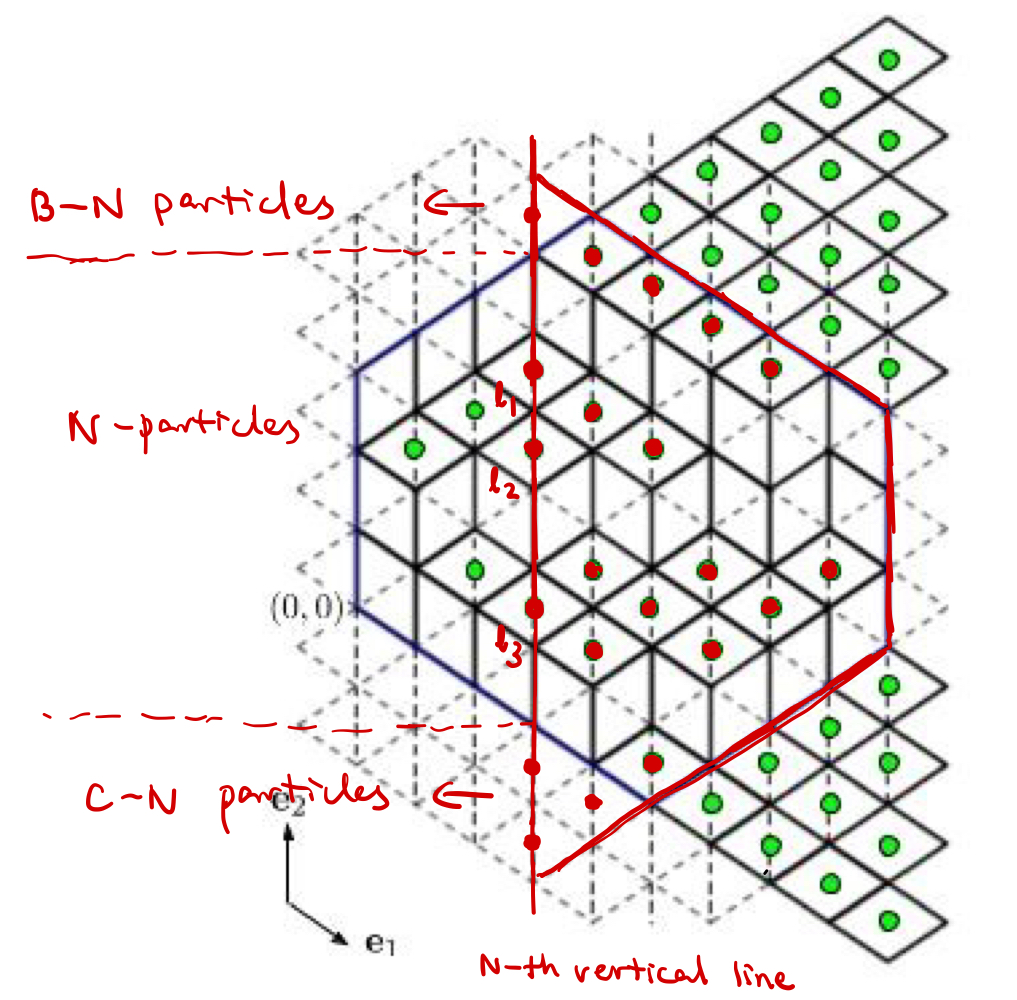
\includegraphics[scale=0.2]{converse-tiling}
	\end{figure}  
	From the picture, we can see the following several facts:
	(\romannumeral 1) Focused on the $n$-th vertical line, the left hand side of it is a tiling from the left to the right, and the right hand side of it is a tiling from the right to the left if we extend the tiling region as the picture does.\\
	(\romannumeral 2) The left hand side(green dots) is a tiling from $(0,0)$ to $(N,\lambda^{\ell})$, while the right hand side(red dots) is a tiling from $(0,0)$ to $(B+C-N,\lambda^{\prime})$, if we look at it in the opposite direction(from the right to the left). Here, $\lambda^{\prime}$ is a new partition that we will investigate in the next paragraph. For now we can easily observe that the extended $N$-$th$ vertical line, or the $(B+C-N)$-$th$ vertical line from the right to the left, contains $B+C-N$ particles. There are $B-N$ particles above and $C-N$ particles below the hexagon region, which are specified in the picture. Also, the hexagon region contains $N$ particles of the original tiling from the left to the right.\\
	(\romannumeral 3) From the construction of the tiling and the ``converse tiling'' in the opposite direction, we can find that there is a bijection between tiling from $(N,\lambda^{\ell})$ to $(B+C,\mu)$ and tiling from $(0,0)$ to $(B+C-N,\lambda^{\prime})$. Therefore, to compute the number of tilings from $(N,\lambda^{\ell})$ to $(B+C,\mu)$ is equivalent to compute the number of tilings from $(0,0)$ to $(B+C-N,\lambda^{\prime})$.\\
	\par Next, let's find the new partition $\lambda^{\prime}$. In the following proof, we consider the ``converse tiling'' and use the corresponding coordinates. We denote the second coordinates of the particles on the $(B+C-N)$-$th$ vertical line by $y^{B+C-N}_{i}$ from the top to the bottom, $i=1,2,\dots,B+C-N$. Denote $\ell^{\prime}_{i}=y^{B+C-N}_{i}-\frac{1}{2}$, and it's easy to check: 
	$$
	\ell^{\prime}_{i}=
	\begin{cases}
	A+B+C-N-i, &\text{if $1\leqslant i\leqslant B-N$;} \\
	\ell_{i-(B-N)}+C-N, &\text{if $B-N+1\leqslant i\leqslant B$;}\\
	B+C-N-i, &\text{if $B+1\leqslant i\leqslant B+C-N$;}
	\end{cases}
	$$
	Define $\lambda_{i}^{\prime}=\ell_{i}^{\prime}-(B+C-N-i)$, $i=1,2,\dots,B+C-N$, and it is not difficult to check:
	$$
	\lambda^{\prime}_{i}=
	\begin{cases}
	A, &\text{if $i\in I_{1}$;} \\
	\ell_{i-(B-N)}-B+i, &\text{if $i\in I_{2}$;}\\
	0, &\text{if $i\in I_{3}$;}
	\end{cases}
	$$
	where $I_{1}=\llbracket{1,B-N}\rrbracket$, $I_{2}=\llbracket{B-N+1,B}\rrbracket$, $I_{3}=\llbracket{B+1,B+C-N}\rrbracket$. We also denote $I=\llbracket{1,N}\rrbracket$ and $T=\llbracket{1,C-N}\rrbracket$. Then we compute the Schur polynomial $$s_{\lambda^{\prime}}(1^{B+C-N})=\prod_{1\leqslant i<j\leqslant B+C-N}\frac{\lambda^{\prime}_{i}-\lambda_{j}^{\prime}+j-i}{j-i}$$
	The product in the above equality can be divided into the following $6$ parts:
	\begin{align*}
	P_{1} &= \prod_{i<j; i,j\in I_{1}}\frac{\lambda_{i}-\lambda_{j}+j-i}{j-i}=\prod_{i<j; i,j\in I_{1}}\frac{A-A+j-i}{j-i}=1\\
	P_{2} &= \prod_{i\in I_{1},j\in I_{2}}\frac{A-(\ell_{j-(B-N)}-B+j)+j-i}{j-i}=\prod_{i\in I_{1},j\in I_{2}}\frac{A-\ell_{j-(B-N)}+B-i}{j-i}\\ 
	&= \prod_{i\in I_{1},j\in I}\frac{A-\ell_{j}+B-i}{j+B-N-i} = \prod_{j\in I}\frac{(A+B-\ell_{j}-1)!/(A+N-\ell_{j}-1)!}{(j+B-N-1)!/(j-1)!}\\
	P_{3}&=\prod_{i\in I_{1},j\in I_{3}}\frac{A-0+j-i}{j-i}=\prod_{i\in I_{1},j\in I_{3}}\frac{A+j-i}{j-i}\\
	P_{4}&=\prod_{i<j;i,j\in I_{2}}\frac{\lambda^{\prime}_{i}-\lambda_{j}^{\prime}+j-i}{j-i}=\prod_{i<j;i,j\in I_{2}}\frac{\ell_{i-(B-N)}-\ell_{j-(B-N)}}{j-i}\\
	&= \prod_{1\leqslant i<j\leqslant N}\frac{\ell_{i}-\ell_{j}}{j-i}=s_{\lambda^{\ell}}(1^{N})\\
	P_{5}&=\prod_{i\in I_{2},j\in I_{3}}\frac{(\ell_{i-(B-N)}-B+i)+j-i}{j-i}=\prod_{i\in I_{2},j\in I_{3}}\frac{\ell_{i-(B-N)}-B+j}{j-i}\\
	&= \prod_{i\in I,j\in T}\frac{\ell_{i}+j}{j-i+N}=\prod_{i\in I}\frac{(\ell_{i}+C-N)!/\ell_{i}!}{(C-i)!/(N-i)!}\\
	P_{6}&=\prod_{i<j; i,j\in I_{3}}\frac{0-0+j-i}{j-i}=1
	\end{align*}
	Notice that only $P_{2}$ and $P_{5}$ contain the term $\ell_{i}$, and we have 
	\begin{align*}
	P_{2}\cdot P_{5} &= \prod_{i=1}^{N}\frac{(A+B-\ell_{i}-1)!(\ell_{i}+C-N)!}{(A+N-\ell_{i}-1)!\ell_{i}!}\cdot\prod_{i=1}^{N}\frac{(j-1)!(N-i)!}{(j+B-N-1)!(C-i)!}\\
	&=\Big[\prod_{i=1}^{N}\omega(\ell_{i})\Big]\cdot M
	\end{align*} 
	where $$M=\prod_{i=1}^{N}\frac{(j-1)!(N-i)!}{(j+B-N-1)!(C-i)!}$$ and $$\omega(\ell_{i})=\frac{(A+B-\ell_{i}-1)!(\ell_{i}+C-N)!}{(A+N-\ell_{i}-1)!\ell_{i}!}$$
	To sum up,
	\begin{align*}
	\mathbb P(\ell_1,\cdots \ell_N)&=\frac{s_{\lambda^{\ell}}(1^{N})\prod_{k=1}^{6}P_{k}}{s_{\mu}(1^{B+C})}=\frac{(s_{\lambda^{\ell}}(1^{N}))^{2}\cdot P3\cdot P2\cdot P5}{s_{\mu}(1^{B+C})}\\
	&=\prod_{1\leqslant i<j\leqslant N}\frac{(\ell_{i}-\ell_{j})^{2}}{(j-i)^{2}}\cdot\Big[\prod_{i=1}^{N}\omega(\ell_{i})\Big]\cdot M\cdot P_{3}\cdot\frac{1}{s_{\mu}(1^{B+C})}\\
	&=\frac{1}{Z}\prod_{1\leqslant i <j\leqslant N}(\ell_{i}-\ell_{j})^{2}\prod_{i=1}^{N}\omega(\ell_{i})
	\end{align*}
	where
	\begin{align*}
	Z^{-1}=\frac{M\cdot P_{3}}{s_{\mu}(1^{B+C})}\prod_{1\leqslant i<j\leqslant N}\frac{1}{(j-i)^{2}}
	\end{align*}
	and the expression of $M$, $s_{\mu}(1^{B+C})$, $P_{3}$, and $\omega(\ell_{i})$ are given above.
	
	\subsection*{Problem 12}

From the previous problem, we have the probability distribution
\begin{equation}\label{Eqn1}
	\mathbb{P}(\ell_1, \dots, \ell_N) = \frac{1}{Z} \prod_{1 \leq i < j \leq N} (\ell_i - \ell_j)^2 \prod_{i = 1}^Nw(\ell_i),
\end{equation}
where $l_i=x_id_2\sqrt{L}+d_1L$, and
\begin{equation}\label{Eqn2}
	w(l_i) = \frac{(A+B-l_i-1)! (l_i+C-N)!}{(A+N-l_i-1)!l_i!} 
\end{equation}
By Sterling's Approximation,
\begin{align*}
	&(A+B-l_i-1)!  \\
	=& \left[(a+b-d_1)L-x_id_2\sqrt{L}-1\right]! \\
	\to& \sqrt{2\pi\left[(a+b-d_1)L-x_id_2\sqrt{L}-1\right]} 
	\exp \left[-(a+b-d_1)L+x_id_2\sqrt{L}+1\right] \\
	& \exp\left[ \left((a+b-d_1)L-x_id_2\sqrt{L}-1\right) \ln{\left((a+b-d_1)L-x_id_2\sqrt{L}-1\right)} \right] 
\end{align*}
Using Taylor expansion,
\begin{align*}
	&\ln{\left((a+b-d_1)L-x_id_2\sqrt{L}-1\right)} \\
	=& \ln(a+b-d_1)L-\frac{x_id_2}{(a+b-d_1)\sqrt{L}}-\frac{x_i^2d_2^2}{2(a+b-d_1)^2L}+O(\frac{1}{L})
\end{align*}
The exponent becomes
\begin{align*}
	&\left((a+b-d_1)L-x_id_2\sqrt{L}-1\right) \ln{\left((a+b-d_1)L-x_id_2\sqrt{L}-1\right)}\\
	=& \left((a+b-d_1)L-x_id_2\sqrt{L}-1\right) 
	\left( \ln(a+b-d_1)L-\frac{x_id_2}{(a+b-d_1)\sqrt{L}}-\frac{x_i^2d_2^2}{2(a+b-d_1)^2L}+O(\frac{1}{L}) \right) \\
	=& (a+b-d_1)L\ln(a+b-d_1)L - x_id_2 \sqrt{L}\ln(a+b-d_1)L-x_id_2\sqrt{L} + \frac{x_i^2d_2^2}{2(a+b-d_1)} + O(\frac{1}{\sqrt{L}})
\end{align*}
Similarly, we can calculate the exponent for other factorials
\begin{align*}
	& \left( (c+d_1)L+x_id_2\sqrt{L}-N \right) \ln\left( (c+d_1)L+x_id_2\sqrt{L}-N \right)\\
	=& (c+d_1)L \ln(c+d_1)L+x_id_2\sqrt{L}\ln(c+d_1)L-N\ln(c+d_1)L+x_id_2\sqrt{L}-N-\frac{x_i^2d_2^2}{2(c+d_1)} + O(\frac{1}{\sqrt{L}})
\\
	& \left( (a-d_1)L-x_id_2\sqrt{L}+N-1 \right) \ln\left( (a-d_1)L-x_id_2\sqrt{L}+N-1 \right)\\
	=& (a-d_1)L \ln(a-d_1)L-x_id_2\sqrt{L}\ln(a-d_1)L+(N-1)\ln(a-d_1)L-x_id_2\sqrt{L}\\
	&\qquad +(N-1)-\frac{x_i^2d_2^2}{2(a-d_1)} + O(\frac{1}{\sqrt{L}})
\\
	& \left( d_1L+x_id_2\sqrt{L} \right)\ln\left( d_1L+x_id_2\sqrt{L} \right) \\
	=& d_1L\ln(d_1L)+x_id_2\sqrt{L}\ln(d_1L)+x_id_2\sqrt{L}+\frac{x_i^2d_2^2}{2d_1} + O(\frac{1}{\sqrt{L}})
\end{align*}
Summing the four exponents yields
\begin{align*}
	&(a+b-d_1)L\ln(a+b-d_1)L + ((c+d_1)L-N) \ln(c+d_1)L\\
	&\qquad- ((a-d_1)L-N+1)\ln(a-d_1)L - d_1L\ln(d_1L) \\
	&\qquad- x_id_2 \sqrt{L}\ln(a+b-d_1)L + x_id_2\sqrt{L}\ln(c+d_1)L + x_id_2\sqrt{L}\ln(a-d_1)L - x_id_2\sqrt{L}\ln(d_1L)\\
	&\qquad+ \frac{x_i^2d_2^2}{2(a+b-d_1)} +\frac{x_i^2d_2^2}{2(c+d_1)} -\frac{x_i^2d_2^2}{2(a-d_1)} -\frac{x_i^2d_2^2}{2d_1} + O(\frac{1}{\sqrt{L}})
\end{align*}
Substitution into the weight function yields the limit
\begin{align*}
	w(l_i) \to& \ L^{(b+c)L-1}
	\frac{(a+b-d_1)^{(a+b-d_1)L} (c+d_1)^{(c+d_1)L-N}}{(a-d_1)^{(a-d_1)L-N+1} d_1^{d_1L}} \exp\left(2N-(b+c)L\right)\\
	&\qquad\cdot
	\exp\left(\frac{x_i^2d_2^2}{2}(\frac{1}{a+b-d_1}+\frac{1}{c+d_1}-\frac{1}{a-d_1}-\frac{1}{d_1})\right)\\
	&\qquad\cdot
	\exp\left(x_id_2\sqrt{L} \ln\frac{(c+d_1)(a-d_1)}{(a+b-d_1)d_1}\right)
\end{align*}
Solving equations
\begin{align*}
	\frac{(c+d_1)(a-d_1)}{(a+b-d_1)d_1} =& \ 1 \\
	 \frac{x_i^2d_2^2}{2}(\frac{1}{a+b-d_1}+\frac{1}{c+d_1}-\frac{1}{a-d_1}-\frac{1}{d_1}) =& -\frac{x_i^2}{2}
\end{align*}
we obtain
\begin{align*}
	d_1 &= \frac{ac}{b+c} \\
	d_2 &= \sqrt{\frac{abc(a+b+c)}{(b+c)^3}}
\end{align*}

	
	\subsection*{Problem 13}

$$\omega(l_i) = \frac{(A + B - l_i - 1)! \times (l_i + C - N)!}{(A + N - l_i - 1)! \times l_i!}$$

We can rewrite $\omega(l_i)$ as
$$(A + B - l_i - 1)! = \frac{(A + B)!}{\prod_{0 \leq k \leq l_i}(A + B - k)}$$
$$ (C - N + l_i)! = (C - N - 1)! \prod_{0 \leq k \leq l_i}(C - N + k)$$
$$(A + N - l_i - 1)! = \frac{(A + N -1)!}{\prod_{0 \leq k \leq l_i}(A + N -1 -k)}$$

Also,

$$\frac{(A +B - l_i 1)! (l_i + C - N)!}{(A + N - l_i - 1)! l_i!}$$
$$=\frac{(A + B)!}{\prod_{0 \leq k \leq l_i} (A + B - k)} \times (C - N - 1)! \prod_{0 \leq k \leq l_i} (C - N + k) \times \frac{\prod_{0 \leq k \leq l_i}(A + N - 1 - k)}{(A + N - 1)!} \times \frac{1}{l_i!}$$

Now, $N$, and the $l_i$ are constants, while $A$, $B$, $C$ all go to infinity, with $\frac{A_n C_n}{B_n}$ going to $t$. Rewrite the above as

$$\frac{(A+ B)! \times (C-N - 1)!}{(A + N- 1)!} \times \prod_{0 \leq k \leq l_i} \frac{(C-N + k)\times (A+N-1-k)}{(A + B - k)}$$

Consider the limit

$$\lim_{n \rightarrow \infty} \prod_{0 \leq k \leq l_i} \frac{(C_n - N + k)\times (A_n + N - 1 - k)}{(A_n + B_n - k)} = \prod_{0 \leq k \leq l_i} \lim_{n \rightarrow \infty} \frac{(C_n - N + k)\times (A_n + N - 1 - k)}{(A_n + B_n - k)}$$

$$\lim_{n \rightarrow \infty} \frac{(C_n - N + k)\times (A_n + N - 1 - k)}{(A_n + B_n - k)} = \lim_{n \rightarrow \infty}\frac{\frac{(C_n - N + k) \times (A_n + N - 1 - k)}{(A_n C_n )}}{\frac{(A_n + B_n - k)}{(A_n C_n)}}$$

$$= \lim_{n \rightarrow \infty} \frac{( 1 - (N - k)}{C_n} \times \frac{\frac{( 1 - (N - 1 - k)}{A_n}}{\frac{1}{C_n} + \frac{1}{t} + \frac{k}{A_n C_n}} = \lim_{n \rightarrow \infty} \frac{1}{\frac{1}{t}} = t$$

Then

$$\lim_{n \rightarrow \infty} \prod_{0 \leq k \leq l_i} \frac{(C_n - N + k)\times (A_n+N-1-k)}{(A_n + B_n - k)} = t^{l_i + 1} $$\\

Now, we want to find

$$\lim_{n \rightarrow \infty} \frac{(A_n+ B_n)! \times (C_n-N - 1)!}{(A_n + N- 1)!}$$
$$\log \left( \frac{(A+B)! \times (C - N - 1)!}{(A + N - 1)!}\right) 
= \log((A+B)!) + \log((C-N-1)!) - \log(( A + N - 1)!)$$ \\

By Stirling's Formula:

$$\log(n!) = n\log(n) - n + O(\log(n))$$

...

	\subsection*{Problem 14}
	By Cauchy identity, we have $$\sum_{\lambda}s_{\lambda}(a^{N})s_{\lambda}(b^{N})=\prod_{1\leqslant i,j\leqslant N}(1-ab)^{-1}=(1-ab)^{-N^2}$$ Therefore, $z_{N}(a,b)=(1-ab)^{-N^2}$. By Problem 4, Schur symmetric function is a homogeneous polynomial with degree $|\lambda|$. Thus, $s_{\lambda}(a^{N})=a^{\sum_{i=1}^{n}\lambda_{i}}s_{\lambda}(1^{N})$ and $s_{\lambda}(b^{N})=b^{\sum_{i=1}^{n}\lambda_{i}}s_{\lambda}(1^{N})$. Then,
	\begin{align*}
		\mathbb{P}(\lambda)&\propto s_{\lambda}(a^{N})\cdot s_{\lambda}(b^{N})=(ab)^{\sum_{i=1}^{n}\lambda_{i}}(s_{\lambda}(1^{N}))^{2}=(ab)^{\sum_{i=1}^{N}(\ell_{i}+i-N)}\Big[\prod_{1\leqslant i<j\leqslant N}\frac{\lambda_{i}-\lambda_{j}+j-i}{j-i}\Big]^{2}\\&=(ab)^{(\sum_{i=1}^{n}\ell_{i})-\frac{1}{2}N(N-1)}\Big[\prod_{1\leqslant i<j\leqslant N}\frac{\ell_{i}-\ell_{j}}{j-i}\Big]^{2}\\&=(ab)^{-\frac{1}{2}N(N-1)}\prod_{1\leqslant i<j\leqslant N} \frac{1}{(j-i)^{2}}\cdot \prod_{1\leqslant i<j\leqslant N}(\ell_{i}-\ell_{j})^{2}\cdot\prod_{i=1}^{N}(ab)^{\ell_{i}}
	\end{align*}
Let $x_{i}=\frac{\ell_{i}}{n}$, we have $(ab)^{-\ell_{i}}=e^{-\frac{\ell_{i}}{n}}=e^{-x_{i}}$. Denote $\omega(x_{i})=e^{-x_{i}}$ and then
$$\rho(x_{1},x_{2},\dots,x_{N})\propto\prod_{1\leqslant i<j \leqslant N}(x_{i}-x_{j})^2\prod_{i=1}^{N}\omega(x_{i})$$
Thus, the constant $Z_{N}=\int_{0}^{\infty}\dots\int_{0}^{\infty}\prod_{1\leqslant i<j \leqslant N}(x_{i}-x_{j})^2\prod_{i=1}^{N}e^{-x_{i}}=\frac{1}{N!}\prod_{i=0}^{N-1}(i!)^2$, and this follows from Selberg's Integral.


\section{Couplings}

	\subsection*{Problem 15}
	
	We will prove the following lemma, of which the two lemmas 3.1 and 3.2 are immediate consequences. In particular, Lemma 3.1 is the special case when $g^b = g^t$, and Lemma 3.2 is the case when $\vec{x} = \vec{x}'$ and $\vec{y} = \vec{y}'$. We argue in analogy to Lemma 5.6 in Dimitrov-Matestki.
	
	\begin{lemma*}
		Fix $k \in \mathbb{N}$, $T_0, T_1 \in \mathbb{Z}$ with $T_0 < T_1$, and two functions $g^b, g^t: \llbracket T_0, T_1 \rrbracket  \rightarrow [-\infty, \infty)$ with $g^b\leq g^t$. Also fix $\vec{x}, \vec{y}, \vec{x}', \vec{y}' \in \mathfrak{W}_k$, such that $g^b(T_0)\leq x_i$, $g^b(T_1)\leq y_i$, $g^t(T_0)\leq x_i'$, $g^t(T_1)\leq y_i'$, and $x_i\leq x_i'$, $y_i\leq y_i'$ for $1\leq i\leq k$. Assume that $\Omega_{avoid}(T_0, T_1, \vec{x}, \vec{y}, \infty,g^b)$ and $\Omega_{avoid}(T_0, T_1, \vec{x}', \vec{y}', \infty,g^t)$ are both non-empty. Then there exists a probability space $(\Omega, \mathcal{F}, \mathbb{P})$, which supports two $\llbracket 1, k \rrbracket$-indexed Bernoulli line ensembles $\mathfrak{L}^t$ and $\mathfrak{L}^b$ on $\llbracket T_0, T_1 \rrbracket$ such that the law of $\mathfrak{L}^{t}$ {\big (}resp. $\mathfrak{L}^b${\big )} under $\mathbb{P}$ is given by $\mathbb{P}_{avoid, Ber}^{T_0, T_1, \vec{x}', \vec{y}', \infty, g^t}$ {\big (}resp. $\mathbb{P}_{avoid, Ber}^{T_0, T_1, \vec{x}, \vec{y}, \infty, g^b}${\big )} and such that $\mathbb{P}$-almost surely we have $\mathfrak{L}_i^t(r) \geq \mathfrak{L}^b_i(r)$ for all $i = 1,\dots, k$ and $r \in \llbracket T_0, T_1 \rrbracket$.
	\end{lemma*}

	\begin{proof} We split the proof into two steps.\\
	
	\textbf{Step 1.} We first aim to construct a Markov chain $(X^n,Y^n)_{n\geq 0}$, with \\$X^n\in \Omega_{avoid}(T_0,T_1,\vec{x},\vec{y},\infty,g^b)$, $Y^n\in \Omega_{avoid}(T_0,T_1,\vec{x}',\vec{y}',\infty,g^t)$, with initial distribution given by the maximal paths
	\begin{align*}
	& X^0_1(t)=(x_1+t-T_0) \wedge y_1,\quad && Y^0_1(t)=(x_1'+t-T_0) \wedge y_1'\\
	& X^0_k(t)=(x_k+t-T_0) \wedge y_k \wedge X^0_{k-1}(t), \quad && Y^0_k(t)=(x_k'+t-T_0) \wedge y_k' \wedge Y^0_{k-1}(t).
	\end{align*}
	for $t\in\llbracket T_0, T_1\rrbracket$. We want this chain to have the following properties: 
	\begin{enumerate}[label=(\arabic*)]
		
		\item $(X^n)_{n\geq 0}$ and $(Y^n)_{n\geq 0}$ are both Markov in their own filtrations,
		
		\item $(X^n)$ is irreducible and has as an invariant distribution the uniform measure $\mathbb{P}_{avoid,Ber}^{T_0,T_1,\vec{x},\vec{y},\infty,g^b}$,
		
		\item $(Y^n)$ is irreducible and has invariant distribution $\mathbb{P}_{avoid,Ber}^{T_0,T_1,\vec{x}',\vec{y}',\infty,g^t}$,
		
		\item $X^n_i\leq Y^n_i$ on $\llbracket T_0, T_1\rrbracket$ for all $n\geq 0$ and $1\leq i \leq k$.
		
	\end{enumerate}

	\noindent This will allow us to conclude convergence of $X^n$ and $Y^n$ to these two uniform measures.
	
	We specify the dynamics of $(X^n, Y^n)$ as follows. At time $n$, we uniformly sample a segment $\{t\}\times[z, z+1]$, with $t\in\llbracket T_0, T_1\rrbracket$ and $z\in\llbracket x_k,y_1'-1\rrbracket$. We also flip a fair coin, with $\mathbb{P}(\textrm{heads})=\mathbb{P}(\textrm{tails})=1/2$. We update $X^n$ and $Y^n$ using the following procedure. For all points $s\neq t$, we set $X^{n+1}(s) = X^n(s)$. If $T_0 < t < T_1$ and $X^n_i(t-1)=z$ and $X^n_i(t+1)=z+1$ (note that this implies $X^n_i(t)\in\{z,z+1\}$), then we set
	\[
	X^{n+1}_i(t) = \begin{cases}
		z+1, & \textrm{if heads},\\
		z, & \textrm{if tails},
	\end{cases}
	\]
	assuming that this move does not cause $X^{n+1}_i(t)$ to fall below $g^b(t)$. In all other cases, we leave $X^{n+1}_i(t)=X^n_i(t)$. We update $Y^n$ using the same rule, with $g^t$ in place of $g^b$. [Maybe add a figure here.] We will verify below in the proof of (4) that $X^n$ and $Y^n$ are in fact non-intersecting for all $n$, but we assume this for now.
	
	It is easy to see that $(X^n,Y^n)$ is a Markov chain, since at each time $n$, the value of $(X^{n+1},Y^{n+1})$ depends only on the current state $(X^n,Y^n)$, and not on the time $n$ or any of the states prior to time $n$. Moreover, the value of $X^{n+1}$ depends only on the state $X^n$, not on $Y^n$, so $(X^n)$ is a Markov chain in its own filtration. The same applies to $(Y^n)$. This proves the property (1) above.
	
	We now argue that $(X^n)$ is each irreducible. Observe that the initial distribution $X^0$ is by construction maximal, in the sense that for any $Z\in \Omega_{avoid}(T_0,T_1,\vec{x},\vec{y}\infty,g^b)$, we have $Z_i \leq X^0_i$ for all $i$. Thus to reach $Z$ from the initial state $X_0$, we only need to move the paths downward, and there is no danger of the paths $X_i$ crossing when we do so. We start by ensuring $X^n_k = Z_k$. We successively sample segments which touch $Z_k$ at each point in $\llbracket T_0,T_1\rrbracket$ where $Z_k$ differs from $X_k$, and choose the appropriate coin flips until the two agree on all of $\llbracket a,b\rrbracket$. We repeat this procedure for $X^n_i$ and $Z^i$, with $i$ descending. Since each of these samples and flips has positive probability, and this process terminates in finitely many steps, the probability of transitioning from $X^n$ to $Z$ after some number of steps is positive. The same reasoning applies to show that $(Y^n)$ is irreducible.
	
	To see that the uniform measure $\mathbb{P}_{avoid,Ber}^{T_0,T_1,\vec{x},\vec{y},\infty,g^b}$ on $\Omega_{avoid}(T_0,T_1,\vec{x},\vec{y},\infty,g^b)$ is invariant for $(X^n)$, fix any line ensemble $\omega\in\Omega_{avoid}(T_0,T_1,\vec{x},\vec{y},\infty,g^b)$. For simplicity, write $\mu$ for the uniform measure and $N=|\Omega_{avoid}(T_0,T_1,\vec{x},\vec{y},\infty,g^b)|$ for the (finite) number of allowable ensembles. Then for all ensembles $\tau\in\Omega_{avoid}(T_0,T_1,\vec{x},\vec{y},\infty,g^b)$, $\mu(\tau) = 1/N$. Hence
	\begin{align*}
	\sum_\tau \mu(\tau)\mathbb{P}(X^{n+1} = \omega\,|\,X^n = \tau) &= \frac{1}{N}\sum_\tau \mathbb{P}(X^{n+1} = \omega\,|\,X^n = \tau)\\
	&= \frac{1}{N}\sum_\tau \mathbb{P}(X^{n+1} = \tau\,|\,X^n = \omega)\\
	&= \frac{1}{N}\cdot 1 = \mu(\omega).
	\end{align*}
	The second equality is clear if $\tau=\omega$. Otherwise, note that $\mathbb{P}(X_{n+1} = \omega\,|\,X_n = \tau) \neq 0$ if and only if $\tau$ and $\omega$ differ only in one indexed path (say the $i$th) at one point $t$, where $|\tau_i(t)-\omega_i(t)|=1$, and this condition is also equivalent to $\mathbb{P}(X^{n+1} = \tau\,|\,X^n = \omega) \neq 0$. If $X^n=\tau$, there is exactly one choice of segment $\{t\}\times[z,z+1]$ and one coin flip which will ensure $X^{n+1}_i(t)=\omega(t)$, i.e., $X^{n+1}=\omega$. Conversely, if $X^n=\omega$, there is one segment and one coin flip which will ensure $X^{n+1}=\tau$. Since the segments are sampled uniformly and the coin flips are fair, these two conditional probabilities are in fact equal. This proves (2), and an analogous argument proves (3).
	
	Lastly, we argue that $X^n_i\leq Y^n_i$ for all $n\geq 0$ and $1\leq i\leq k$. The same argument will prove that $X^n_{i+1}\leq X^n_i$ for all $n,i$, so that $X^n$ is in fact non-intersecting for all $n$, and likewise for $Y^n$. This is of course true at $n=0$. Suppose it holds at some $n\geq 0$.Then since the update rule can only change the values of $X_i$ and $Y_i$ at a single point $t$, we see that in order for the inequality to be violated at time $n+1$, we must have some $t$ with $T_0 < t < T_1$ such that $X^n_i(t)=Y^n_i(t)$. In order for an update to be applied, we must also have either $X^n_i(t+1) - X^n_i(t-1) = 1$, or $Y^n_i(t+1) - Y^n_i(t-1) = 1$. Now the basic idea is that after any update, if $X^n$ increases, then so must $Y^n$, and if $Y^n$ decreases, then so must $X^n$. We make this precise by considering all possible updates.
	
	First suppose $X^n_i(t+1) - X^n_i(t-1) = 1$. If $X^n_i(t) = X^n_i(t+1)$, then the only possible nontrivial update results in $X^{n+1}_i(t) = X^n_i(t) - 1 \leq Y^n_i(t) - 1 \leq Y^{n+1}_i(t)$. If there is no update because $X^n_i(t)-1 < g^b(t)$, then there can also be no decrease in $Y$ since this implies $Y^n_i(t)-1 < g^b(t) \leq g^t(t)$. If $X^n_i(t) = X^n_i(t-1)$, then the only update is $X^n_i(t+1) = X^n_i(t)+1$, which forces $Y^n_i(t+1) = Y^n_i(t)+1$ by the assumption that $X^n_i\leq Y^n_i$. Then $X^{n+1}_i(t) = Y^{n+1}_i(t) = X^n_i(t) + 1$, and we still have $X^{n+1}_i(t)\leq Y^{n+1}_i(t)$. 
	
	Now assume $Y^n_i(t+1)-Y^n_i(t-1) = 1$. If $Y^n_i(t) = Y^n_i(t-1)$, then the only update is $Y^{n+1}_i(t) = Y^n_i(t) + 1 \geq X^n_i(t) + 1 \geq X^n_i(t)$. On the other hand if $Y^n_i(t) = Y^n_i(t+1)$, then we must also have $X^n_i(t) = X^n_i(t+1)$, so that the only nontrivial update is $Y^{n+1}_i(t) = X^{n+1}_i(t) = Y^n_i(t) - 1$. If this update is suppressed because $Y^n_i(t)-1 < g^t(t)$, then we still have $X^{n+1}_i(t) \leq X^n_i(t) = Y^n_i(t) = Y^{n+1}_i(t)$. In all cases, we see that $X^{n+1}_i\leq Y^{n+1}_i$, proving (4) by induction.\\
	
	\textbf{Step 2.} It follows from (2) and (3) that $(X^n)_{n\geq 0}$ and $(Y^n)_{n\geq 0}$ converge weakly to $\mathbb{P}_{avoid,Ber}^{T_0,T_1,\vec{x},\vec{y},\infty,g^b}$ and $\mathbb{P}_{avoid,Ber}^{T_0,T_1,\vec{x}',\vec{y}',\infty,g^t}$ respectively, c.f. Norris, Theorem 1.8.3. In particular, $(X^n)$ and $(Y^n)$ are tight, so $(X^n,Y^n)_{n\geq 0}$ is tight as well. By Prohorov's theorem, it follows that $(X^n,Y^n)$ is relatively compact. Let $(n_m)$ be a sequence such that $(X^{n_m},Y^{n_m})$ converges weakly. Then by the Skorohod representation theorem (see Billingsley, Theorem 6.7), it follows that there exists a probability space $(\Omega,\mathcal{F},\mathbb{P})$ supporting $C(\llbracket 1, k\rrbracket \times \llbracket T_0, T_1\rrbracket)$-valued random variables $\mathfrak{X}^n$, $\mathfrak{Y}^n$ and $\mathfrak{X},\mathfrak{Y}$ such that
	\begin{enumerate}[label=(\arabic*)]
		
		\item The law of $(\mathfrak{X}^n,\mathfrak{Y}^n)$ under $\mathbb{P}$ is the same as that of $(X^n,Y^n)$,
		
		\item $\mathfrak{X}^n(\omega) \longrightarrow \mathfrak{X}(\omega)$ for all $\omega\in\Omega$,
		
		\item $\mathfrak{Y}^n(\omega) \longrightarrow \mathfrak{Y}(\omega)$ for all $\omega\in\Omega$.
		
	\end{enumerate}

	In particular, (1) implies that $\mathfrak{X}^{n_m}$ has the same law as $X^{n_m}$, which converges weakly to $\mathbb{P}_{avoid,Ber}^{T_0,T_1,\vec{x},\vec{y},\infty,g^b}$. It follows from (2) and the uniqueness of limits that $\mathfrak{X}$ has law $\mathbb{P}_{avoid,Ber}^{T_0,T_1,\vec{x},\vec{y},\infty,g^b}$. Similarly, $\mathfrak{Y}$ has law $\mathbb{P}_{avoid,Ber}^{T_0,T_1,\vec{x}',\vec{y}',\infty,g^t}$. Moreover, condition (4) in Step 1 implies that $\mathfrak{X}^n_i \leq \mathfrak{Y}^n_i$, $\mathbb{P}$-a.s., so $\mathfrak{X}_i \leq \mathfrak{Y}_i$ for $1\leq i\leq k$, $\mathbb{P}$-a.s. Thus we can take $\mathfrak{L}^b := \mathfrak{X}$ and $\mathfrak{L}^t := \mathfrak{Y}$.
	
	\end{proof}


\section{Avoiding Bernoulli line ensembles}

	\section*{Problem 16}
	Let $\Omega(0,T,\bar x^T, \bar y ^T)$ be the set of all non intersecting Bernoulli line ensembles from $\bar x^T$ to $\bar y^T$ then we may find that for each line ensemble $\mathfrak{B}\in \Omega(0,T,\bar x^T,\bar y^T)$ with $\mathfrak B=(B_1,...,B_k)$, we may define $\lambda_i(\mathfrak B):=(B_1(i),B_2(i),...,B_k(i))$. 
This is a partition since by the definition of avoiding Bernoulli line ensembles, we have the inequality $B_\alpha(i)>B_\beta(i)$ if $\alpha<\beta$. 
Now because $B_\alpha(i+1)-B_\alpha(i)\in \{0,1\}$ we know that $B_\alpha(i+1)\geq B_\alpha(i)$ but also since $B_\alpha(i+1)\in \mathbb{Z}$ and $B_{\alpha+1}<B_\alpha(i+1)$ (strictly) by the earlier stated inequality, we know that$B_{\alpha+1}+1\leq B_\alpha(i+1)$ and so we find that 
\[B_{\alpha+1}(i+1)\leq B_\alpha(i)\leq B_\alpha(i+1)\]
We therefore find that for all $i$, $\lambda_i\preceq \lambda_{i+1}$. Note that if we plug in $i=0$, we get $\lambda_0=\bar x^T$ and $\lambda_T=\bar y^T$.

Now, let us define the set 
\[TB_{\kappa/\mu}^T:=\{(\lambda_0,...,\lambda_T)\mid \lambda_0=\mu, \lambda_T=\kappa, \lambda_i\preceq\lambda_{i+1}\}\] 
Now, if we take $f:\Omega(0,T,\bar x^T, \bar y ^T)\to TB_{\kappa/\mu}^T$ with $f(\mathfrak{B})= (\lambda_0(\mathfrak{B}),\cdots \lambda_T(\mathfrak{B}))$. We find that this function is in fact a bijection. 

First, as proof for injectivity, suppose that there are two Bernoulli line ensembles, $\mathfrak{B}, \mathfrak{B}'\in \Omega(0,T,\bar x^T, \bar y ^T)$ such that $\mathfrak{B}\neq \mathfrak{B'}$.
Because Bernoulli line ensembles are determined by their values at integer times, we find that this would imply that there exists some $(q,r)$ such that $0\leq r\leq T$, $0\leq q \leq k$ and $B_q(r)\neq B'_q(r)$ where $B_q$ and $B_q'$ are components of $\mathfrak{B}$ and $\mathfrak{B'}$ respectively. 
This implies that $\lambda_r(\mathfrak B)\neq \lambda_r'(\mathfrak{B'})$, and so we have injectivity. 

Now, surjectivity follows since for any $\bar\lambda=(\lambda_0,...,\lambda_T)$ we may define $\mathfrak{B}(\bar{\lambda})=(B_1(\bar\lambda),...,B_k(\bar\lambda))$ where $B_r(\bar\lambda)(i)=\lambda_i^r$ where $\lambda_i^r$ is the $i$\textit{th} entry of $\lambda_r$. The restrictions on $TB_{\kappa/\mu}^T$ ensure that each $\mathfrak{B}(\bar\lambda)\in \Omega(0,T,\bar x^T,\bar y^T)$, and so $f(\mathfrak B(\bar{\lambda}))=(\lambda_0,\cdots \lambda_T)$ by the definition $\mathfrak{B}(\bar\lambda)$. 

We can proceed to use Macdonald Chapter 1, Section 5, Equation (11) to show that, in a very similar way to practice problem 10, we get that 
\[s_{\kappa/\mu}(1^T)=\sum_{(\nu)}\prod_{i=1}^n s_{\nu^{(i)}/\nu^{i-1}}=\sum_{(\nu)} 1=\lvert TB_{\mu/\kappa}^T\rvert\]

Therefore, we can find that 
\begin{align*}
\pr(L_1(\lfloor tT\rfloor)=\lambda_1,\cdots, L_k(\lfloor tT\rfloor)=\lambda_k)
&=\frac{\lvert \Omega(0,\lfloor Tt\rfloor, \bar x^T, \lambda)\rvert\cdot \lvert \Omega(\lfloor Tt\rfloor ,T, \lambda, \bar y^T)\rvert}{\lvert \Omega(0, T, \bar x^T, \bar y^T)\rvert}\\
&=\frac{s_{\lambda/\bar x^T}(1^{\floor{Tt}})\cdot s_{\bar y^T/\lambda}(1^{T-\floor{Tt}})}{s_{\bar y^T/\bar x^T}(1^T)}
\end{align*}

Now, if we use the Jacobi-Trudi formula on this expression and the identity from Macdonald, page 26 i.e. that $h_r(1^n)=\binom{n+k-1}{k}$, we get the resulting equation 
\begin{align*}
\pr(L_1(\lfloor tT\rfloor)=\lambda_1,\cdots, L_k(\lfloor tT\rfloor)=\lambda_k)
&=\frac{\det\left(h_{\lambda_i^T-x_j^T+j-i}(1^{\floor{tT}})\right)_{1=i,j}^k\cdot\det\left(h_{y_i^T-\lambda_j^T+j-i}(1^{T-\floor{Tt}})\right)_{1=i,j}^k}{\det\left(h_{\lambda_i^T-x_j^T+j-i}(1^T)\right)_{1=i,j}^k}\\
&=\frac{\det\left(\frac{\left(\lambda_i^T-x_j^T+j-i+\floor{tT}-1\right)!}{\left(\floor{Tt}-1\right)!\left(\lambda_i^T-x_j^T+j-i\right)!}\right)_{i,j=1}^k\det\left(\frac{\left(y_i^T-\lambda_j^T+j-i+T-\floor{tT}-1\right)!}{\left(T-\floor{Tt}-1\right)!\left(y_i^T-\lambda_j^T+j-i\right)!}\right)_{i,j=1}^k}{\det\left(\frac{\left(y_i^T-x_j^T+j-i+T-1\right)!}{\left(T-1\right)!\left(y_i^T-x_j^T+j-i\right)!}\right)_{i,j=1}^k}
\end{align*}

Now we can find using Sterling's formula that this expression is equal in the limit to 
\[
\frac{\det\left(\frac{\sqrt{2\pi}(\lambda_i^T-x_j^T+j-i+\floor{tT}-1)^{\lambda_i^T-x_j^T+j-i+\floor{tT}-1/2}e^{-\lambda_i^T+x_j^T-j+i-\floor{tT}+1}}{\sqrt{2\pi}(\floor{tT}-1)^{\floor{Tt}-1/2}e^{-\floor{Tt}+1}\cdot \sqrt{2\pi}(\lambda_i^T-x_j^T+j-i)^{\lambda_i^T-x_j^T+j-i+1/2}e^{-\lambda_i^T+x_j^T-j+i}}\right)_{1=i,j}^k
\det\left(\frac{\left(y_i^T-\lambda_j^T+j-i+T-\floor{tT}-1\right)!}{\left(T-\floor{Tt}-1\right)!\left(y_i^T-\lambda_j^T+j-i\right)!}\right)_{i,j=1}^k}
{\det\left(\frac{\sqrt{2\pi}(y_i^T-x_j^T+j-i+{T}-1)^{y_i^T-x_j^T+j-i+{T}-1/2}e^{-y_i^T+x_j^T-j+i-{T}+1}}{\sqrt{2\pi}({T}-1)^{{T}-1/2}e^{-{T}+1}\cdot \sqrt{2\pi}(y_i^T-x_j^T+j-i)^{\lambda_i^T-x_j^T+j-i+1/2}e^{-\lambda_i^T+x_j^T-j+i}}\right)_{1=i,j}^k}
\]
\[
=\frac{
	\det\left(\frac{
		(\lambda_i-x_j^T+j-i+\floor{tT}-1)^{\lambda_i-x_j^T+j-i+\floor{tT}-1/2}}{\sqrt{2\pi}(\floor{tT}-1)^{\floor{Tt}-1/2}(\lambda_i-x_j^T+j-i)^{\lambda_i-x_j^T+j-i+1/2}}\right)_{1=i,j}^k
	\det\left(\frac{(y_i^T-\lambda_j+j-i+T-\floor{tT}-1)^{y_i^T-\lambda_j+j-i+T-\floor{tT}-1/2}}{\sqrt{2\pi}(T-\floor{tT}-1)^{T-\floor{Tt}-1/2}(y_i^T-\lambda_j^T+j-i)^{y_i^T-\lambda_j+j-i+1/2}}\right)_{1=i,j}^k
	}
{\det\left(\frac{
		(y_i^T-x_j^T+j-i+T-1)^{y_i^T-x_j^T+j-i+{T}-1/2}}{\sqrt{2\pi}(T-1)^{T-1/2}(y_i^T-x_j^T+j-i)^{y_i^T-x_j^T+j-i+1/2}}\right)_{1=i,j}^k}
\]

Now if we take $\lambda_i=z_i\sqrt{T}+ptT$ and we consider each of the determinants individually (for the sake of the margins of this document), we find that the expression is equal to $ABC^{-1}$ where
\begin{align*}
A&=\lim_{T\to\infty}(2\pi)^{-\frac k2}\det
	\left(e^{(\sqrt{T}(z_i-a_j)+T(t+pt))\log(\sqrt{T}(z_i-a_j)+T(t+pt))-tT\log(tT)-((z_i-a_j)\sqrt{T}+ptT)\log((z_i-a_j)\sqrt{T}+ptT)}
	\right)_{1=i,j}^k\\
	&=\lim_{T\to\infty}(2\pi)^{-\frac k2}\det\left(e^{T\left(\left(\frac{z_i-a_j}{\sqrt{T}}+pt+t\right)\left(\log\left(\frac{z_i-a_j}{(t)\sqrt T}+p+1\right)+\log (tT)\right)-t\log(tT)-\left(\frac{z_i-a_j}{\sqrt{T}}+pt\right)\left(\log\left(\frac{z_i-a_j}{t\sqrt T}+p\right)+\log(tT)\right)\right)}\right)_{1=i,j}^k\\
	&=\lim_{T\to\infty}(2\pi)^{-\frac k2}\det\left(e^{T\left(\left(\frac{z_i-a_j}{\sqrt{T}}+pt\right)\log(\frac{\frac{z_i-a_j}{t\sqrt{T}}+p+1}{\frac{z_i-a_j}{t\sqrt{T}}+p})+t\log\left(\frac{z_i-a_j}{t\sqrt{T}}+p+1\right)\right)}
	\right)_{1=i,j}^k\\
	&=\lim_{T\to\infty}(2\pi)^{-\frac k2}\det\left(e^{Tt\log(\frac{z_i-a_j}{t\sqrt{T}}+p+1)}\right)_{1=i,j}^k
	\\
	B&=\lim_{T\to\infty} (2\pi)^{-\frac k2}
	\det\left(e^{\left(
	\sqrt{T}(b_i-z_i)
	\right)}
	\right)_{1=i,j}^k
\end{align*}

	\section*{Lemmas from Section 3.2}
	
	\begin{lemma}\label{LemmaHalfS4} Fix $p \in (0,1)$, $T \in \mathbb{N}$ and $x, y\in \mathbb{Z}$ such that $T \geq y-x \geq 0$, and suppose that $\ell$ has distribution $\mathbb{P}^{0,T,x,y}_{Ber}$. Let $M_1, M_2 \in \mathbb{R}$ be given. Then we can find $W_0 = W_0(p,M_2 - M_1) \in \mathbb{N}$ such that for $T \geq W_0$, $x \geq M_1 T^{1/2}$, $y \geq pT + M_2 T^{1/2}$ and $s \in [0,T]$ we have
		\begin{equation}\label{halfEq1S4}
		\mathbb{P}^{0,T,x,y}_{Ber}\Big( \ell(s)  \geq \frac{T-s}{T} \cdot M_1 T^{1/2} + \frac{s}{T} \cdot \big(p T + M_2 T^{1/2}\big) - T^{1/4} \Big) \geq \frac{1}{3}.
		\end{equation}
	\end{lemma}

	\begin{proof}
		
		Define $A = \lfloor MT_1^{1/2}\rfloor$ and $B = \lfloor pT + M_2 T^{1/2}\rfloor$. Then since $A\leq x$ and $B\leq y$, it follows from Lemma 3.1 that there is a probability space with measure $\mathbb{P}_0$ supporting random variables $\mathfrak{L}_1$ and $\mathfrak{L}_2$, whose laws under $\mathbb{P}_0$ are $\mathbb{P}^{0,T,A,B}_{Ber}$ and $\mathbb{P}^{0,T,x,y}_{Ber}$ respectively, and $\mathbb{P}_0$-a.s. we have $\mathfrak{L}_1\leq \mathfrak{L}_2$. Thus
		\begin{align*}
		&\mathbb{P}^{0,T,x,y}_{Ber}\Big( \ell(s)  \geq \frac{T-s}{T} \cdot M_1 T^{1/2} + \frac{s}{T} \cdot \big(p T + M_2 T^{1/2}\big) - T^{1/4} \Big)\\
		= \; & \mathbb{P}_0\Big( \mathfrak{L}_2(s)  \geq \frac{T-s}{T} \cdot M_1 T^{1/2} + \frac{s}{T} \cdot \big(p T + M_2 T^{1/2}\big) - T^{1/4} \Big)\\
		\geq \; & \mathbb{P}_0\Big( \mathfrak{L}_1(s)  \geq \frac{T-s}{T} \cdot M_1 T^{1/2} + \frac{s}{T} \cdot \big(p T + M_2 T^{1/2}\big) - T^{1/4} \Big)\\
		= \; & \mathbb{P}^{0,T,A,B}_{Ber}\Big( \ell(s)  \geq \frac{T-s}{T} \cdot M_1 T^{1/2} + \frac{s}{T} \cdot \big(p T + M_2 T^{1/2}\big) - T^{1/4} \Big).
		\end{align*}
		Since upright paths on $\llbracket 0,T\rrbracket \times \llbracket A,B\rrbracket$ are equivalent to upright paths on $\llbracket 0,T\rrbracket \times \llbracket 0, B-A\rrbracket$ shifted vertically by $A$, the last line is equal to
		\[
		\mathbb{P}^{0,T,0,B-A}_{Ber}\Big( \ell(s) + A  \geq \frac{T-s}{T} \cdot M_1 T^{1/2} + \frac{s}{T} \cdot \big(p T + M_2 T^{1/2}\big) - T^{1/4} \Big).
		\]
		Now we consider the coupling provided by Theorem 3.3. We have another probability space $(\Omega,\mathcal{F},\mathbb{P})$ supporting a random variable $\ell^{(T,B-A)}$ whose law under $\mathbb{P}$ is that of $\ell$, and a Brownian bridge $B^\sigma$. Then 
		\begin{align*}
		&\mathbb{P}^{0,T,0,B-A}_{Ber}\Big( \ell(s) + A  \geq \frac{T-s}{T} \cdot M_1 T^{1/2} + \frac{s}{T} \cdot \big(p T + M_2 T^{1/2}\big) - T^{1/4} \Big)\\
		= \; & \mathbb{P}\Big( \ell^{(T,B-A)}(s) + A \geq \frac{T-s}{T} \cdot M_1 T^{1/2} + \frac{s}{T} \cdot \big(p T + M_2 T^{1/2}\big) - T^{1/4} \Big)\\
		= \; & \mathbb{P}\Big( \Big[\ell^{(T,B-A)}(s) - \sqrt{T} B^\sigma_{s/T} - \frac{s}{T}\cdot(B-A)\Big] + \sqrt{T}B^\sigma_{s/T} \geq -A-\frac{s}{T}\cdot(B-A) \\
		&\qquad\qquad + \frac{T-s}{T} \cdot M_1 T^{1/2} + \frac{s}{T} \cdot \big(p T + M_2 T^{1/2}\big) - T^{1/4} \Big).
		\end{align*}
		Recalling the definitions of $A$ and $B$, we can rewrite the quantity on the right hand side in the last expression and bound it by
		\begin{align*}
		\frac{T-s}{T}\cdot(M_1T^{1/2}-A) + \frac{s}{T}\cdot(pT + M_2T^{1/2} - B) - T^{1/4} &\leq  \frac{T-s}{T} + \frac{s}{T} - T^{1/4}\\
		& = -T^{1/4} + 1.
		\end{align*}
		Thus
		\begin{align*}
		&\mathbb{P}^{0,T,0,B-A}_{Ber}\Big( \ell(s) + A  \geq \frac{T-s}{T} \cdot M_1 T^{1/2} + \frac{s}{T} \cdot \big(p T + M_2 T^{1/2}\big) - T^{1/4} \Big)\\
		\geq \; & \mathbb{P}\Big( \Big[\ell^{(T,B-A)}(s) - \sqrt{T} B^\sigma_{s/T} - \frac{s}{T}\cdot(B-A)\Big] + \sqrt{T}B^\sigma_{s/T} \geq -T^{1/4} + 1 \Big)\\
		\geq \; & \mathbb{P}\Big( \sqrt{T}B^\sigma_{s/T} \geq 0 \quad \mathrm{and} \quad \Delta(T,B-A) < T^{1/4} - 1 \Big)\\
		\geq \; & \mathbb{P}\left( B^\sigma_{s/T} \geq 0 \right) - \mathbb{P}\left( \Delta(T,B-A) \geq T^{1/4} - 1 \right)\\
		= \; & \frac{1}{2} - \mathbb{P}\left( \Delta(T,B-A) \geq T^{1/4} - 1 \right).
		\end{align*}
		For the second inequality, we used the fact that the quantity in brackets is bounded in absolute value by $\Delta(T,B-A)$. The third inequality follows by splitting the event $\{B^\sigma_{s/T}\geq 0\}$ into cases and applying subadditivity. It remains to bound the second term on the last line. Applying Chebyshev's inequality and Theorem 3.3, we obtain constants $C,a,\alpha$ depending only on $p$ such that
		\begin{align*}
		\mathbb{P}\left( \Delta(T,B-A) \geq T^{1/4} - 1 \right) & \leq e^{-a(T^{1/4} - 1)} \ex\Big[ e^{a\Delta(T,B-A)} \Big]\\
		&\leq C \exp\left[ -a(T^{1/4}-1) + \alpha(\log T)^2 + \frac{|B-A-pT|^2}{T} \right]\\
		&\leq C \exp\left[ -a(T^{1/4}-1) + \alpha(\log T)^2 + (M_2-M_1)^2 + \frac{1}{T} \right]\\
		&= O(e^{-T^{1/4}}).
		\end{align*}
		Thus we can choose $W_0$ large enough, depending on $p$ and $M_2-M_1$, so that if $T \geq W_0$, then this probability does not exceed $1/6$. Combining this with the above inequalities completes the proof.
		
	\end{proof}

	\begin{lemma}\label{LemmaMinFreeS4} Fix $p \in (0,1)$, $T \in \mathbb{N}$ and $y\in \mathbb{Z}$ such that $T \geq y \geq 0$, and suppose that $\ell$ has distribution $\mathbb{P}^{0,T,0,y}_{Ber}$. Let $M > 0$ and $\epsilon > 0$ be given. Then we can find $W_1=W_1(M,p, \epsilon) \in \mathbb{N}$ and $A=A(M,p, \epsilon) > 0$ such that for $T \geq W_1$, $ y \geq p T -  MT^{1/2}$ we have
		\begin{equation}\label{minFree1S4}
		\mathbb{P}^{0,T,0,y}_{Ber}\Big( \inf_{s \in [ 0, T]}\big( \ell(s) -  ps \big) \leq -AT^{1/2} \Big) \leq \epsilon.
		\end{equation}
	\end{lemma}
	
	\begin{proof}
		
		As in the previous proof, it follows from Lemma 3.1 that
		\[
		\mathbb{P}^{0,T,0,y}_{Ber}\Big( \inf_{s \in [ 0, T]}\big( \ell(s) -  ps \big) \leq -AT^{1/2} \Big) \leq \mathbb{P}^{0,T,0,B}_{Ber}\Big( \inf_{s \in [ 0, T]}\big( \ell(s) -  ps \big) \leq -AT^{1/2} \Big),
		\]
		where $B=\lfloor pT - MT^{1/2}\rfloor$. By Theorem 3.3, there is a probability space $(\Omega,\mathcal{F},\mathbb{P})$ supporting a random variable $\ell^{(T,B)}$ whose law under $\mathbb{P}$ is that of $\ell$, and a Brownian bridge $B^\sigma$ with variance $\sigma^2 = p(1-p)$. Therefore
		\begin{align*}
		&\mathbb{P}^{0,T,0,B}_{Ber}\Big( \inf_{s \in [ 0, T]}\big( \ell(s) -  ps \big) \leq -AT^{1/2} \Big) = \mathbb{P}\Big( \inf_{s \in [ 0, T]}\big( \ell^{(T,B)}(s) -  ps \big) \leq -AT^{1/2} \Big)\\
		\leq \; & \mathbb{P}\Big( \inf_{s \in [ 0, T]}  \sqrt{T}B^\sigma_{s/T} \leq -\frac{1}{2}AT^{1/2} \Big) + \mathbb{P}\Big( \sup_{s\in [0,T]} \Big|\sqrt{T} B^\sigma_{s/T} + ps - \ell^{(T,B)}(s) \Big| \geq \frac{1}{2}AT^{1/2} \Big)\\
		\leq \; & \mathbb{P}\Big( \max_{s\in[0,T]} \sqrt{T}B^\sigma_{s/T} \geq \frac{1}{2}AT^{1/2} \Big) + \mathbb{P}\Big(\Delta(T,B) \geq \frac{1}{2}AT^{1/2} - MT^{1/2} - 1\Big).
		\end{align*}
		For the first term in the last line, we used the fact that $B^\sigma$ and $-B^\sigma$ have the same distribution. For the second term, we used the fact that
		\begin{align*}
		\sup_{s\in[0,T]}\Big| ps - \frac{s}{T}\cdot B \Big| &\leq \sup_{s\in[0,T]}\Big| ps - \frac{pT-MT^{1/2}}{T}\cdot s \Big| + 1 = MT^{1/2} + 1.
		\end{align*} To estimate the first term, note that $\sqrt{T}B^\sigma_{s/T} = \sigma\sqrt{T}(W_{s/T} - W_1)$, where $W$ is a standard Brownian motion on $[0,1]$. Hence
		\begin{align*}
		\mathbb{P}\Big( \max_{s\in[0,T]} \sqrt{T}B^\sigma_{s/T} \geq \frac{1}{2}AT^{1/2} \Big) &\leq \mathbb{P}\Big( \sigma\max_{s\in[0,T]} \sqrt{T}\,W_{s/T} \geq \frac{1}{4}AT^{1/2} \Big) + \mathbb{P}\Big( \sigma\sqrt{T}\,W_1 \leq -\frac{1}{4}AT^{1/2} \Big)\\
		&= \mathbb{P}\Big( \sigma\big|\sqrt{T}\,W_{T/T}\big| \geq \frac{1}{4}AT^{1/2} \Big) + \mathbb{P}\Big( \sigma W_1 \leq -\frac{1}{4}A \Big)\\
		&= 3\,\mathbb{P}\Big( W_1 \geq \frac{A}{4\sqrt{p(p-1)}} \Big).
		\end{align*} 
		The equality in the second line follows from the reflection principle, since $\sqrt{T}\,W_{s/T}$ is a standard Brownian motion on $[0,T]$, and the third line follows by symmetry. Since $W_1\sim\mathcal{N}(0,1)$, we can choose $A$ large enough depending on $p$ and $\epsilon$ so that this probability is bounded above by $\epsilon/2$. 
		
		For the second term, it follows from Theorem 3.3 and Chebyshev's inequality that
		\begin{align*}
		\mathbb{P}\Big(\Delta(T,B) \geq \Big(\frac{A}{2} - M\Big)T^{1/2} - 1\Big) &\leq C\exp\Big[-a\Big(\frac{A}{2}- M\Big)T^{1/2} + a + \alpha(\log T)^2 + M^2 + \frac{1}{T}\Big].
		\end{align*}
		If we take $A > 2M$, then this is $O(e^{-T^{1/2}})$, and then we can find $W_1$ large enough depending on $M,p,\epsilon$ so that this term is also $\leq\epsilon/2$ for $T\geq W_1$. Adding the two terms gives (4).
		
	\end{proof}

	\begin{lemma}\label{LemmaTailS4}Fix $p \in (0,1)$, $T \in \mathbb{N}$ and $x, y\in \mathbb{Z}$ such that $T \geq y-x \geq 0$, and suppose that $\ell$ has distribution $\mathbb{P}^{0,T,x,y}_{Ber}$. Let $M_1,M_2 > 0$ be given. Then we can find $W_2 = W_2(M_1,M_2,p) \in \mathbb{N}$ such that for $T \geq W_2$, $ x \geq -M_1T^{1/2}$, $ y \geq pT -  M_1T^{1/2}$ we have
		\begin{equation}\label{halfEq2S4}
		\mathbb{P}^{0,T,x,y}_{Ber}\bigg( \ell( T/2 )  \geq \frac{M_2T^{1/2} + p T}{2} - T^{1/4} \bigg) \geq (1/2) (1 - \Phi^{v}(M_1 + M_2) ),
		\end{equation}
		where $\Phi^{v}$ is the cumulative distribution function  of a Gaussian random variable with mean $0$ and variance $v = p(1-p)/4$.
	\end{lemma}
	
	\begin{proof}
		
		We have
		\begin{align*}
		\mathbb{P}^{0,T,x,y}_{Ber}\bigg( \ell( T/2 )  \geq \frac{M_2T^{1/2} + p T}{2} - T^{1/4} \bigg) &\geq \mathbb{P}^{0,T,0,B-A}_{Ber}\bigg( \ell( T/2 ) + A  \geq \frac{M_2T^{1/2} + p T}{2} - T^{1/4} \bigg)\\
		&= \mathbb{P}\bigg( \ell^{(T,B-A)}( T/2 ) + A  \geq \frac{M_2T^{1/2} + p T}{2} - T^{1/4} \bigg),
		\end{align*}
		with $A = \lfloor -M_1T^{1/2}\rfloor$, $B = \lfloor pT-M_1T^{1/2}\rfloor$, and $\mathbb{P}$, and $\ell^{(T,B-A)}$ provided by Theorem 3.3. If $B^\sigma$ is as in Theorem 3.3, we can rewrite the expression on the second line as
		\begin{align*}
		& \mathbb{P}\bigg( \bigg[\ell^{(T,B-A)}( T/2 ) -\sqrt{T}\,B^\sigma_{1/2} - \frac{B-A}{2}\bigg] + \sqrt{T}\,B^\sigma_{1/2}  \geq -A - \frac{B-A}{2} + \frac{M_2T^{1/2} + p T}{2} - T^{1/4} \bigg).
		\end{align*}
		We have
		\begin{align*}
		-A - \frac{B-A}{2} + \frac{M_2T^{1/2} + p T}{2} - T^{1/4} & \leq M_1T^{1/2} + 1 - \frac{pT-1}{2} + \frac{M_2T^{1/2} + p T}{2} - T^{1/4}\\
		&\leq (M_1 + M_2)T^{1/2} - T^{1/4} + 2.
		\end{align*}
		Thus the probability in question is bounded below by
		\begin{align*}
		& \mathbb{P}\bigg( \bigg[\ell^{(T,B-A)}( T/2 ) -\sqrt{T}\,B^\sigma_{1/2} - \frac{B-A}{2}\bigg] + \sqrt{T}\,B^\sigma_{1/2}  \geq (M_1 + M_2)T^{1/2} - T^{1/4} + 2 \bigg)\\
		\geq \; & \mathbb{P}\bigg( \sqrt{T}\,B^\sigma_{1/2} \geq (M_1 + M_2)T^{1/2} \quad \mathrm{and} \quad \Delta(T,B-A) < T^{1/4} - 2 \bigg)\\
		\geq \; & \mathbb{P}\big( B^\sigma_{1/2} \geq M_1 + M_2 \big) - \mathbb{P}\big( \Delta(T,B-A) \geq T^{1/4} - 2 \big).
		\end{align*}
		Note that $B^\sigma_{1/2} = \sigma(W_{1/2} - \frac{1}{2}W_1)$ for a standard Brownian motion $W$ on $[0,1]$. Thus $B^\sigma_{1/2}$ is Gaussian with mean 0 and variance $\sigma^2(1/2-(1/2)^2) = \sigma^2/4$. In particular, the first term in the last line is equal to
		\[
		1 - \Phi^v(M_1+M_2),
		\]
		where $\Phi^v$ is the cdf for a Gaussian random variable with mean 0 and variance $v=\sigma^2/4 = p(1-p)/4$. For the second term, the same argument as in the proof of Lemma 3.5 shows that it is $O(e^{-T^{1/4}})$. In particular, we can choose $W_2$ depending on $M_1,M_2$, and $p$ so that the second term is less than 1/2 the first term for $T\geq W_2$. This proves (5).
		
	\end{proof}

	\begin{lemma}\label{LemmaAwayS4} Fix $p \in (0,1)$, $T \in \mathbb{N}$ and $x, y\in \mathbb{Z}$ such that $T \geq y-x \geq 0$, and suppose that $\ell$ has distribution $\mathbb{P}^{0,T,x,y}_{Ber}$. Then we can find $W_3 = W_3(p) \in \mathbb{N}$ such that for $T \geq W_3$, $ x \geq T^{1/2}$, $ y \geq pT +  T^{1/2}$
		\begin{equation}\label{awayS4}
		\mathbb{P}^{0,T,x,y}_{Ber}\Big( \inf_{s \in [0,T]} \big( \ell(s) -ps \big)+ T^{1/4} \geq 0 \Big) \geq \frac{1}{2} \left(1 - \exp\left(-\frac{2}{p(1-p)}\right)\right).
		\end{equation}
	\end{lemma}
	
	\begin{proof}
		
		We have
		\begin{align*}
		& \mathbb{P}^{0,T,x,y}_{Ber}\Big( \inf_{s \in [0,T]} \big( \ell(s) -ps \big)+ T^{1/4} \geq 0 \Big) \\
		\geq \; & \mathbb{P}^{0,T,0,B-A}_{Ber}\Big( \inf_{s \in [0,T]} \big( \ell(s) + A -ps \big)+ T^{1/4} \geq 0 \Big)\\
		= \; & \mathbb{P}\Big( \inf_{s \in [0,T]} \big( \ell^{(T,B-A)}(s) -ps \big) \geq - T^{1/4} - A \Big)\\
		\geq \; & \mathbb{P}\Big( \inf_{s \in [0,T]} \big( \ell^{(T,B-A)}(s) - \frac{s}{T}\cdot(B-A) \big) \geq - T^{1/4} - T^{1/2} + 2 \Big),
		\end{align*}
		with $A = \lfloor T^{1/2}\rfloor$, $B = \lfloor pT + T^{1/2}\rfloor$, and $\mathbb{P}$, and $\ell^{(T,B-A)}$ provided by Theorem 3.3. In the last line, we used the facts that $|A-T^{1/2}|\leq 1$ and $|p-(B-A)/T|\leq 1$. With $B^\sigma$ as in Theorem 3.3, the last line is bounded below by
		\begin{align*}
		&\mathbb{P}\Big( \inf_{s\in[0,T]} \sqrt{T}\,B^\sigma_{s/T} \geq - T^{1/2} \quad \mathrm{and} \quad \Delta(T,B-A) < T^{1/2} - 2 \Big)\\
		\geq \; & \mathbb{P}\Big( \max_{s\in[0,T]} B^\sigma_{s/T} \leq 1 \Big) - \mathbb{P}\Big( \Delta(T,B-A) \geq T^{1/2} - 2 \Big).
		\end{align*}
		To compute the first term, note that if $B^1$ is a Brownian bridge with variance 1 on $[0,1]$, then $\sigma \sqrt{T}\,B^1_{s/T}$ on $[0,T]$ has the same distribution as $B^\sigma_{s/T}$. Hence
		\begin{align*}
		\mathbb{P}\Big( \max_{s\in[0,T]} \sqrt{T}\,B^\sigma_{s/T} \leq T^{1/2} \Big) &= 1 - \mathbb{P}\Big( \max_{s\in[0,T]} \sqrt{T}\,B^1_{s/T} \geq T^{1/2}/\sigma \Big) = 1 - e^{-2(T^{1/2}/\sigma)^2/T}\\ 
		&= 1- \exp\left(-\frac{2}{p(1-p)}\right).
		\end{align*}
		For the second equality, see (3.40) in Chapter 4 of Karatzas \& Shreve, \textit{Brownian Motion and Stochastic Calculus}.
		
		The second term is $O(e^{-T^{1/2}})$ by the same argument as in the proof of Lemma 3.5, so we can choose $W_3$ large enough depending on $p$ so that this term is less than 1/2 the first term for $T\geq W_3$. This implies (6).
		
		
	\end{proof}

	We need the following definition for our next result. For a function $f \in C[a,b]$ we define its {\em modulus of continuity} by
	\begin{equation}\label{MOCS4}
	w(f,\delta) = \sup_{\substack{x,y \in [a,b]\\ |x-y| \leq \delta}} |f(x) - f(y)|.
	\end{equation}
	\begin{lemma}\label{MOCLemmaS4}Fix $p \in (0,1)$, $T \in \mathbb{N}$ and $y\in \mathbb{Z}$ such that $T \geq y \geq 0$, and suppose that $\ell$ has distribution $\mathbb{P}^{0,T,0,y}_{Ber}$. For each positive $M$, $\epsilon$ and $\eta$, there exist a $\delta(\epsilon, \eta, M) > 0$ and $W_4 = W_4(M, p, \epsilon, \eta) \in \mathbb{N}$ such that  for $T \geq W_4$ and $|y - pT| \leq MT^{1/2}$ we have
		\begin{equation}\label{MOCeqS4}
		\mathbb{P}^{0,T,0,y}_{Ber}\Big( w\big({f^\ell},\delta\big) \geq \epsilon \Big) \leq \eta,
		\end{equation}
		where $f^\ell(u) = T^{-1/2}\big(\ell(uT) - puT\big)$  for $u \in [0,1]$.
	\end{lemma}
	
	\begin{proof}
		
		We have
		\[
		\mathbb{P}^{0,T,0,y}_{Ber}\Big( w\big({f^\ell},\delta\big) \geq \epsilon \Big) = \mathbb{P}\Big( w\big(f^{\ell^{(N,y)}},\delta\big) \geq \epsilon \Big),
		\]
		with $\mathbb{P}$, $f^{\ell^{(N,y)}}$. If $B^\sigma$ is the Brownian bridge provided by Theorem 3.3, then
		\begin{align*}
		w\big(f^{\ell^{(N,y)}},\delta\big) &= T^{-1/2} \sup_{\substack{x,y \in [0,1]\\ |x-y| \leq \delta}} \Big| \ell^{(N,y)}(xT) - pxT - \ell^{(N,y)}(yT) + pyT \Big|\\
		&\leq T^{-1/2} \sup_{\substack{x,y \in [0,1]\\ |x-y| \leq \delta}} \Big| \sqrt{T}\,B^\sigma_x + xy - pxT - \sqrt{T}\,B^\sigma_y - y^2 + pyT \Big|\\
		&\qquad + T^{-1/2}\cdot\Big|\sqrt{T}\,B^\sigma_x + xy - \ell^{(N,y)}(xT)\Big| + T^{-1/2}\cdot\Big|\sqrt{T}\,B^\sigma_y + y^2 - \ell^{(N,y)}(yT)\Big|\\
		&\leq \sup_{\substack{x,y \in [0,1]\\ |x-y| \leq \delta}} \Big| B^\sigma_x - B^\sigma_y + T^{-1/2} (y-pT)(x-y)\Big| + 2T^{-1/2}\Delta(T,y)\\
		&\leq w\big(B^\sigma,\delta\big) + M\delta + 2T^{-1/2}\Delta(T,y).
		\end{align*}
		The last line follows from the assumption that $|y-pT|\leq MT^{1/2}$. Thus
		\begin{align*}
		\mathbb{P}\Big( w\big(f^{\ell^{(N,y)}},\delta\big) \geq \epsilon \Big) &\leq \mathbb{P}\Big( w\big(B^\sigma,\delta\big) + M\delta + 2T^{-1/2}\Delta(T,y) \geq \epsilon \Big)\\
		&\leq \mathbb{P}\Big( w\big(B^\sigma,\delta\big) + M\delta \geq \epsilon/2 \Big) + \mathbb{P}\Big( \Delta(T,y) \geq \epsilon\, T^{1/2}/2 \Big).
		\end{align*}
		The last term is $O(e^{-T^{1/2}})$ by the argument in the proof of Lemma 3.5, so we can choose $W_4$ large enough depending on $M,p,\epsilon,\eta$ so that this term is $\leq\eta/2$ for $T\geq W_4$. Since $B^\sigma$ is a.s. uniformly continuous on the compact interval $[0,1]$, $w(B^\sigma,\delta) \to 0$ as $\delta\to 0$. Thus we can find $\delta_0>0$ small enough depending on $\epsilon,\eta$ so that $w(B^\sigma,\delta_0) < \epsilon/2$ with probability at least $1-\eta/2$. Then with $\delta = \min(\delta_0, \epsilon/4M)$, the first term is $\leq\eta/2$ as well. This implies (8).
		
	\end{proof}
	
	
\end{document}
